% !TeX document-id = {e7fef4b9-afbc-4e81-94aa-c4847183d047}
% !BIB program = biber
\documentclass[10pt, times, conference, letterpaper]{IEEEtran}
\usepackage{nopageno}

%\usepackage[T1]{fontenc}
%\usepackage{amsfonts}
\usepackage{amsmath}
\let\openbox\relax
\usepackage{amsthm}
\usepackage[cmintegrals]{newtxmath}
\usepackage{bm}

\usepackage[dvipsnames]{xcolor}
\usepackage{graphicx}
\usepackage{tikz}
\usepackage{varwidth}
\usetikzlibrary{arrows.meta, calc, fit, positioning, shapes.misc}

\usepackage{etoolbox}
\usepackage[binary-units, per-mode=symbol]{siunitx}
\robustify\bfseries
\sisetup{detect-all, range-phrase=--, range-units=single, detect-weight=true,detect-inline-weight=math}

\makeatletter
\let\MYcaption\@makecaption
\makeatother

\usepackage[font=footnotesize]{subcaption}

\makeatletter
\let\@makecaption\MYcaption
\makeatother

\usepackage[basic]{complexity}
\usepackage[super,negative]{nth}

\usepackage[british]{babel}
\usepackage{csquotes}

\usepackage{booktabs}
\usepackage[
activate={true,nocompatibility},
final,
tracking=true,
kerning=true,spacing=true
]{microtype}
\microtypecontext{spacing=nonfrench}

%% Fix indent in new section...
\newcommand{\subparagraph}{}
\usepackage{titlesec}
\titlespacing*{\section}{0pt}{1.5ex}{0.7ex}
\titlespacing*{\subsection}{0pt}{1.5ex}{0.7ex}
\titlespacing*{\paragraph}{0pt}{1.5ex}{0.7ex}
\titlespacing*{\subsubsection}{0pt}{1.5ex}{0.7ex}
%\titleformat*{\filcenter\scshape}

\usepackage{enumitem}
\setlist[description]{leftmargin=8em,style=nextline}

%bib
\usepackage[style=ieee,maxnames=3,mincitenames=1,maxcitenames=2,maxbibnames=99,
mincrossrefs=99,minxrefs=99,
sortcites,
%backend=bibtex,
uniquelist=false]{biblatex}
\addbibresource{papers-off.bib}
\addbibresource{confs-off.bib}
\addbibresource{books-off.bib}
\addbibresource{rfc.bib}
\addbibresource{misc.bib}

%picky abt et al.
%\usepackage{xpatch}

%\xpatchbibmacro{name:andothers}{%
%	\bibstring{andothers}%
%}{%
%	\bibstring[\emph]{andothers}%
%}{}{}

% emph'd et al. for ieee style
\DefineBibliographyStrings{english}{%
	andothers = {\emph{et al}\adddot}
}
\DeclareFieldFormat[inproceedings]{url}{}
\DeclareFieldFormat[article]{url}{}
\DeclareFieldFormat[inproceedings]{doi}{}
\DeclareFieldFormat[article]{doi}{}
\DeclareFieldFormat[inproceedings]{editor}{}
\DeclareFieldFormat[proceedings]{editor}{}
\DeclareFieldFormat[article]{editor}{}

% Thanks to http://codydunne.blogspot.com/2012/01/suppressing-bibtex-fields-for-specific.html
\AtEveryBibitem{% Clean up the bibtex rather than editing it
	\clearlist{address}
%	\clearfield{date}
%	\clearfield{eprint}
	\clearfield{isbn}
	\clearfield{issn}
	\clearlist{location}
%	\clearfield{month}
	\clearfield{series}
	
	\ifentrytype{book}{}{% Remove publisher and editor except for books
		\clearlist{publisher}
		\clearname{editor}
	}

	\ifentrytype{mics}{}{% Remove publisher and editor except for books
		\clearfield{url}
	}
}

%opening!

%\newcommand{\mytitle}{Improving Direct-Control Reinforcement Learning for Network Intrusion Prevention}
\newcommand{\mytitle}{Protocol-Agnostic DDoS Mitigation through Reinforcement Learning}

\usepackage{url}
\usepackage{hyperref}
\usepackage[nameinlink]{cleveref}
\newcommand{\crefrangeconjunction}{--}
\crefname{table}{table}{tables}

\hypersetup{
	colorlinks,
	citecolor=black,
	filecolor=black,
	linkcolor=black,
	urlcolor=black,
	pdftitle={\mytitle{}},
%	pdfauthor={Kyle A. Simpson, Simon Rogers, Dimitrios P. Pezaros}
	pdfauthor={Anonymous Giraffe, Anonymous Badger, Anonymous Ibex}
}
\newcommand*{\email}[1]{\href{mailto:#1}{\nolinkurl{#1}} } 

\usepackage{titling}
%\settowidth{\thanksmarkwidth}{*}
%\setlength{\thanksmargin}{-\thanksmarkwidth}
%
%%% Enable /thanks
%\IEEEoverridecommandlockouts
%\makeatletter
%\def\footnoterule{\relax%
%	\kern-5pt
%	\hbox to \columnwidth{\hfill\vrule width 0.5\columnwidth height 0.4pt\hfill}
%	\kern4.6pt}
%\makeatother

% make math easy
\newcommand{\acval}[3]{\ensuremath{\operatorname{\hat{q}}(#1, #2, #3)}}
\newcommand{\wvec}[1]{\ensuremath{\bm{w}_{#1}}}

%thm environments
\newtheorem{thm}{Theorem}
\newtheorem{corr}{Corollary}[thm]

\newcommand{\fakepara}[1]{\noindent\textbf{#1:}}

\makeatletter\let\expandableinput\@@input\makeatother

\makeatletter
\DeclareRobustCommand{\rvdots}{%
	\vbox{
		\baselineskip4\p@\lineskiplimit\z@
		\kern-\p@
		\hbox{.}\hbox{.}\hbox{.}
}}
\makeatother

% Official colours!

\definecolor{uofguniversityblue}{rgb}{0, 0.219608, 0.396078}

\definecolor{uofgheather}{rgb}{0.356863, 0.32549, 0.490196}
\definecolor{uofgaquamarine}{rgb}{0.603922, 0.72549, 0.678431}
\definecolor{uofgslate}{rgb}{0.309804, 0.34902, 0.380392}
\definecolor{uofgrose}{rgb}{0.823529, 0.470588, 0.709804}
\definecolor{uofgmocha}{rgb}{0.709804, 0.564706, 0.47451}

\definecolor{uofglawn}{rgb}{0.517647, 0.741176, 0}
\definecolor{uofgcobalt}{rgb}{0, 0.615686, 0.92549}
\definecolor{uofgturquoise}{rgb}{0, 0.709804, 0.819608}
\definecolor{uofgsunshine}{rgb}{1.0, 0.862745, 0.211765}
\definecolor{uofgpumpkin}{rgb}{1.0, 0.72549, 0.282353}
\definecolor{uofgthistle}{rgb}{0.584314, 0.070588, 0.447059}
\definecolor{uofgpillarbox}{rgb}{0.701961, 0.047059, 0}
\definecolor{uofglavendar}{rgb}{0.356863, 0.301961, 0.580392}

\definecolor{uofgsandstone}{rgb}{0.321569, 0.278431, 0.231373}
\definecolor{uofgforest}{rgb}{0, 0.317647, 0.2}
\definecolor{uofgburgundy}{rgb}{0.490196, 0.133333, 0.223529}
\definecolor{uofgrust}{rgb}{0.603922, 0.227451, 0.023529}

\definecolor{inferno0}{rgb}{0.001462 0.000466 0.013866}
\definecolor{inferno64}{rgb}{0.341500 0.062325 0.429425}
\definecolor{inferno128}{rgb}{0.735683 0.215906 0.330245}
\definecolor{inferno192}{rgb}{0.978422 0.557937 0.034931}
\definecolor{inferno255}{rgb}{0.988362 0.998364 0.644924}

\colorlet{lowac}{inferno128}
\colorlet{midac}{inferno192}
\colorlet{highac}{inferno255}

%-------------------------------------%
%-------------------------------------%

\title{\mytitle{}}
\author{
%	Kyle~A.~Simpson\thanks{This work was supported by the Engineering and Physical Sciences Research Council [grant number EP/M508056/1].},
%	Kyle~A.~Simpson,
%	Simon~Rogers,
%	Dimitrios~P.~Pezaros,~\IEEEmembership{Senior~Member,~IEEE,},\\
%	School of Computing Science, University of Glasgow, Glasgow, G12 8RZ, UK\\
%	University of Glasgow, Glasgow, Scotland,\\
%	\email{k.simpson.1@research.gla.ac.uk}
Anonymous Giraffe,
Anonymous Badger,
Anonymous Ibex\\
Unnamed Department, Nowhere\\
\email{giraffe.a@unnamed.com}
}

% Remove date, leave no spacing.
\predate{}
\postdate{}
\date{}

\begin{document}

%% If needed, make urls typewritery
%\urlstyle{tt}

\maketitle

\begin{abstract}
DDoS attacks still cause significant harm to online services to this day.
Their detection is difficult, because like many cybersecurity problems they \emph{evolve}: normal and attack patterns shift due to new protocols and applications.
Such evolution makes it difficult to apply machine learning techniques and defences.

Reinforcement learning (RL) agents manage and monitor system health in an online manner.
Unsupervised, online learning is a key part of overcoming this detection problem.
We present the architecture of a system designed to host such RL agents in a typical network.
Furthermore, we introduce two agents which advance the state-of-the-art in using RL for DDoS mitigation.
Both of these act per flow, in a protocol-agnostic manner for any network topology.
This is supported by an in-depth investigation of feature suitability and empirical evaluation.

Our results show the existence of flow features with high predictive power for bulk TCP and VoIP traffic.
We show that the new agents offer a significant increase in throughput of legitimate TCP traffic for many choices of host density.
\end{abstract}

%\begin{IEEEkeywords}
%	Security services, distributed denial-of-service, software-defined networking, machine learning, reinforcement learning.
%\end{IEEEkeywords}

\section{Introduction}
?? Redo intro to be more system focussed? Needs to be suitably different.

Network anomaly detection and intrusion detection/prevention are continually evolving problems, compounded by the partial, non-\emph{independent and identically distributed} (IID) view of data at each point in the network.
Attacks and anomalous behaviours evolve, becoming more sophisticated or employing new vectors to harm a network or system's confidentiality, integrity, and availability without being detected \cite{DBLP:journals/comsur/BhuyanBK14}.
These attacks and anomalies have measurable consequences and symptoms which allow a skilled analyst to infer new signatures for detection by misuse-based classifiers, but unseen attacks may only be defended against after-the-fact.
This issue is inherent to \emph{misuse-} or \emph{signature-based} intrusion detectors, and it has been long-hoped that \emph{anomaly-based} detectors would surpass this by making effective use of statistical measures \cite{DBLP:journals/comsur/BhuyanBK14}.

While \emph{machine learning} (ML) approaches seem like a sensible fit for this problem, in \citeyear{DBLP:conf/sp/SommerP10} \citeauthor{DBLP:conf/sp/SommerP10} identified the `failure to launch' of ML-based anomaly detection systems---a distinct lack of real-world system deployments \cite{DBLP:conf/sp/SommerP10}.
To quite a large extent, this remains the case today.
These authors posit that their application is made difficult due to significant operational differences from standard ML tasks, including: the high cost of errors and extraordinarily low tolerance for false positives inherent to network intrusion detection \cite{DBLP:conf/ccs/Axelsson99}; a general lack of recent, openly available (and high-quality) training data; and diversity of network traffic across varying timescales combined with significant burstiness \cite{DBLP:journals/ccr/LelandWTW95}.
Above the aggregate level, the constant deployment of new services and new protocols means that traffic is \emph{non-stationary} and displays an evolving notion of normality.
Learning is made harder still by the challenges encountered when learning from unlabelled (often partial) data.
All of these factors greatly inflate the difficulty of the detection problem.

%?? Make it clearer here what problem I specifically want to solve: principally a particular class of DDoS attacks; volume-based DDoS attacks. Amplification attacks are just a specialisation, this can be made more obvious. I think I need to be clearer about the \emph{intended deployment environment} of service hosts (i.e., not ISPs).

For certain classes of problem e.g., volume-based \emph{distributed denial of service} (DDoS) attacks, \emph{reinforcement learning} (RL) offers another perspective.
%?? Unclear explanation of RL here?
RL agents operate by following a \emph{policy} to interact with or control a system, while at the same time using observed performance metrics and deliberate exploration to dynamically improve this policy.
In this way the role of a RL agent differs from that of a standard classifier, adaptively reacting to threats by assuming the role of a feedback loop for network optimisation, typically to safeguard service guarantees.
In a sense, this allows us to ``overcome'' some of the difficulties of the detection problem by monitoring \emph{performance characteristics and consequences} in real-time; by looking for (and controlling) the effect rather than the cause.
Long-term, we expect that the value of RL-based defence systems will be to augment what existing misuse-based solutions can provide, by automatically alerting, recording and controlling what are believed to be illegal system states.
The goal of this work is much less general; we aim to prevent volume-based DDoS attacks with the aid of RL-based techniques (an important goal in its own right), while bringing to light the flexibility and applicability of these techniques in the security domain.
%Whether it takes direct control of the network, or is used indirectly to optimise a key part of another system, more powerful `deep' RL techniques (and well-founded action spaces) aren't yet well explored for network IDS/IPS.
%These range from more modern training algorithms \cite{DBLP:journals/corr/SchulmanWDRK17, DBLP:conf/icml/SchulmanLAJM15}, to evolutionary strategies \cite{DBLP:journals/corr/SalimansHCS17, DBLP:journals/corr/abs-1802-08842}, hierarchical action composition \cite{DBLP:journals/corr/abs-1710-09767}, and competitive multi-agent learning \cite{DBLP:journals/corr/abs-1710-03748}.

To date, there have been few applications of this class of algorithms towards intrusion detection and prevention which make use of their full potential for online control, rather than using them as the basis for a classifier.
We aim to take steps to redress this and establish their proper capabilities, beyond simple ``blind application''.
%?? Expand as required
What approaches do exist are aimed towards the task of adaptive online DDoS mitigation, and rely upon learning to control probabilistic packet drop.
%?? THAT IS A MAJOR CONTRIB, MENTION IT EVERYWHERE YOU CAN

%?? Discuss the most important conclusions before the outline.
We find that the existing work for this task fails to account for congestion-aware traffic (i.e., TCP) and deployment environments with high host density per egress point, achieving poor results due to an overly coarse view of the network.
The approach we identify to remedy this is to make throttling decisions on a per-source basis, and we present the engineering decisions this mandates: updating RL agents from multiple traces per timestep, timed random sequential action computation and a supporting \emph{software-defined network} (SDN) architecture.
In tandem with the development and evaluation of an effective state space and model, we provide the design of a second model inspired by past work on algorithmic DDoS prevention, as an example of the integration of domain-specific knowledge.
Our introduction of per-source decisions improves substantially upon the state-of-the-art when acting upon most internet traffic (i.e., congestion-aware protocols), and we show that our second model achieves excellent performance for high host density in this case.
Crucially, both models remain protocol- and content-agnostic to offer future-proofing against the rollout of future protocols like QUIC \cite{DBLP:conf/sigcomm/LangleyRWVKZYKS17}.
%?? Also algorithmic enhancements such as multiple actions per timestep, 
%?? PROTOCOL-AGNOSTIC -- HOW WILL THESE THINGS COPE WITH QUIC ET AL.?!?!
Briefly, this paper contributes:
\begin{itemize}
%	\item A DDoS mitigation system based on direct-control reinforcement learning, designed for deployment in real-world software-defined networks (\cref{sec:environment-and-rl-algorithm,sec:acting-on-individual-sources}).
%	\item Important weaknesses and flaws in the past design and evaluation of similar techniques \cite{DBLP:journals/eaai/MalialisK15}. We offer a deconstruction and empirical study on their formulation, flaws, and risk factors concerning different traffic distributions---in addition, we demonstrate modifications enabling deployment in real-world software-defined networks (\cref{sec:performance-in-an-emulated-environment}).
	\item Two source-level granularity approaches to RL-driven DDoS prevention (\emph{Instant} and \emph{Guarded} action models), improving upon past aggregate-based models (\cref{sec:ddos-mitigation-with-per-flow-reinforcement-learning}).
	\item An in-depth investigation into suitable features for an automatic DDoS mitigation system, with qualitative and quantitative justification (\cref{sec:rethinking-the-state-space}).
	\item Reactive simulations of HTTP and VoIP web-server traffic, designed to test system characteristics that packet trace playback fails to capture (\cref{sec:a-new-normal}).
	\item An empirical evaluation of our new models against the state-of-the-art in RL-based DDoS mitigation using these new traffic models (\cref{sec:the-results-of-doing-so}), alongside a discussion of security concerns and real-world deployment (\cref{sec:discussion}).
\end{itemize}

\section{Background and Threat Model}
%?? Introduce RL, related definitions etc.

\subsection{Distributed Denial of Service}
%?? DDoS attack variants (leading into characteristics, supporting features). Amplification (UDP \cite{DBLP:conf/ndss/Rossow14}, TCP \cite{DBLP:conf/uss/KuhrerHRH14}), Transit-link (Crossfire \cite{DBLP:conf/sp/KangLG13}, Coremelt \cite{DBLP:conf/esorics/StuderP09}). Mirai botnet's involvement \cite{DBLP:conf/uss/AntonakakisABBB17}.

%?? Explain amplification attack, maybe transit-link?

\emph{Distributed denial of service} (DDoS) attacks are concentrated efforts by many hosts to reduce the availability of a service, typically to inflict financial harm or as an act of vandalism.
Attackers achieve this by either exploiting peculiarities of operating system or application behaviour in \emph{semantic attacks} (e.g., \emph{SYN flooding attacks}), or overwhelming their target through sheer volume of requests or inbound packets (\emph{volume-based attacks}) \cite{DBLP:conf/imc/JonkerKKRSD17}.
Hosts often participate unwillingly, typically having been recruited into a \emph{botnet} by malware infection to be orchestrated from elsewhere \cite{DBLP:conf/uss/AntonakakisABBB17}.

Although there are variations of each class of attack, flooding attacks are the most relevant to our work.
\emph{Amplification attacks} exploit the presence of services who eagerly send large replies in response to small requests, where UDP-based services like DNS and NTP are most exploitable \cite{DBLP:conf/ndss/Rossow14, DBLP:conf/uss/KuhrerHRH14}.
Malicious hosts send many small requests, spoofed to appear as though they originated from the victim, causing many large replies to be sent to the intended target---significantly increasing a botnet's throughput while masking the identity of each participant.
\emph{Transit-link/link-flooding attacks} have been the subject of recent attention, wherein malicious traffic is forwarded across core links needed to reach a target (but not to the target itself) \cite{DBLP:conf/sp/KangLG13, DBLP:conf/esorics/StuderP09}.

\subsection{Reinforcement Learning}\label{sec:reinforcement-learning}
\emph{Reinforcement learning} (RL) is a variant of machine learning concerned with training an agent to choose an optimal sequence of actions for a given task \cite{RL2E}.
We assume at any point in time $t$, an agent knows which \emph{state} it is in ($S_t \in \mathcal{S}$), the set of \emph{actions} which are available to it ($\operatorname{A}(S_t) \subseteq \mathcal{A}$) and numeric \emph{reward} obtained from the last action chosen ($R_t \in \mathbb{R}, A_{t-1} \in \operatorname{A}(S_{t-1})$).
This model of system interaction is best described as a \emph{Markov Decision Process} (MDP).
RL methods combine this information with a current \emph{policy} $\pi$ to determine which action should be taken.
The policy is refined as more decisions and rewards become available, learning adaptively and online.
In practice, this means that agents are able to automatically adapt to evolving problems without operator intervention or a new training corpus.

%?? Include some details of function approximation in the formalisation? I.e. tile coding, stability and convergence guarantees...
We focus on methods based on action value estimates from the current state: let $\operatorname{q}(s, a) \in \mathbb{R}$ denote the estimate of action $a$'s value if it were to be taken in state $s$.
%?? Revisit the maths here, d, dim A, s...
To cope with a continuous state and/or action space, one technique to obtain this value is to employ linear function approximation backed by \emph{tile coding} \cite[pp.\ \numrange{217}{221}]{RL2E}.

\begin{figure}
	\centering
	\begin{subfigure}{0.45\linewidth}
		\resizebox{\linewidth}{!}{
		\begin{tikzpicture}
		\node at (0,0.3){$s = \begin{pmatrix}
			0.7 \\
			0.3
			\end{pmatrix}$};
		\node at (0,-1) {$\bm{x}(s,\cdot) = \begin{Bmatrix}
			T_{1,9}, \\
			T_{2,5}, \\
			T_{\mathit{bias}}
			\end{Bmatrix}$};
		
		\node at (2.5,-0.5) {
			\begin{tikzpicture}
			\draw[step=0.5cm,color=uofgcobalt,opacity=0.7,shift={(0,0)},label=above:{Tiling 0}] (-0.5,-0.5) grid (1,1);
			\fill[uofgcobalt,opacity=0.5] (0.5,-0.5) rectangle (1,0);
			\node[color=uofgcobalt] at (0,1.1) {\footnotesize Tiling 1};
			
			\draw[step=0.5cm,color=uofgpumpkin,opacity=0.9,shift={(0.25,-0.25)},label=above:{Tiling 1}] (-0.5,-0.5) grid (1,1);
			\fill[uofgpumpkin,opacity=0.5,shift={(0.25,-0.25)}] (0,0) rectangle (0.5,0.5);
			\node[color=uofgpumpkin!50!uofgrust] at (0.25,-0.95) {\footnotesize Tiling 2};
			
			\node[circle, black, draw,
			fill, radius=0.5pt, inner sep=0pt,minimum size=1.5pt, label=above:{$s$}] at (0.625,-0.125) {};
%			\filldraw (0.625,-0.125) circle[radius=1.5pt,label=above:{$s$}];

			\draw[->] (-0.25,-0.5)--(-0.25,0.85);
			\draw[->] (-0.25,-0.5)--(1.1,-0.5);
			
			\node at (1,-0.7) {\footnotesize 1};
			\node at (-0.4,0.75) {\footnotesize 1};
			\node at (-0.35,-0.6) {\footnotesize 0};
			\end{tikzpicture}
		};
		
		\end{tikzpicture}
		}
		\caption{Tile Coding\label{fig:tilecode-code}}
	\end{subfigure}%
	\begin{subfigure}{0.45\linewidth}
		\resizebox{\linewidth}{!}{
		\begin{tikzpicture}
		% Top half
		\def\topacs{
			{-0.3,-0.5,-0.1,0.8},
			{0.1,0.1,-0.2,0.3},
			{0.3,0.4,0.2,-0.4}%
		}
	
		\foreach \line [count=\y] in \topacs {
			\foreach \pix [count=\x] in \line {
				\ifthenelse{\lengthtest{\pix pt < 0 pt}}{
					\pgfmathtruncatemacro\lambda{(\pix+1)*100}
					\draw[shift={(-0.7,0)},fill=midac!\lambda!lowac] (0.7*\x,-0.35*\y) rectangle +(0.7,0.35);
				}{
					\pgfmathtruncatemacro\lambda{\pix*100}
					\draw[shift={(-0.7,0)},fill=highac!\lambda!midac] (0.7*\x,-0.35*\y) rectangle +(0.7,0.35);
				}
				\node[shift={(-0.35,0.175)}] at (0.7*\x,-0.35*\y) {\footnotesize \pix};
			}
		}
	
		\draw[xstep=0.7cm,ystep=0.35cm,shift={(0,0)}] (0,-1.06) grid (2.8,0);
		\node[label=left:{$T_{1,9}$},shift={(0,-0.125)}] at (0,0) {}; 
		\node[label=left:{$T_{2,5}$},shift={(0,-0.125)}] at (0,-0.375) {}; 
		\node[label=left:{$T_{\mathit{bias}}$},shift={(0,-0.125)}] at (0,-0.75) {};
		
		% bottom half
		\def\botacs{
			{0.1,0.0,-0.1,0.7}%
		}
	
		\foreach \line [count=\y] in \botacs {
			\foreach \pix [count=\x] in \line {
				\ifthenelse{\lengthtest{\pix pt < 0 pt}}{
					\pgfmathtruncatemacro\lambda{(\pix+1)*100}
					\draw[shift={(-0.7,-1.275)},fill=midac!\lambda!lowac] (0.7*\x,-0.35*\y) rectangle +(0.7,0.35);
				}{
					\pgfmathtruncatemacro\lambda{\pix*100}
					\draw[shift={(-0.7,-1.275)},fill=highac!\lambda!midac] (0.7*\x,-0.35*\y) rectangle +(0.7,0.35);
				}
				\node[shift={(-0.35,-1.1)}] at (0.7*\x,-0.35*\y) {\footnotesize \pix};
			}
		}
	
		\draw[xstep=0.7cm,ystep=0.35cm,shift={(0,-1.275)}] (0,-0.35) grid (2.8,0);
		\node[label=left:{$\mathit{Total}$},shift={(0,-0.175)}] at (0,-1.275) {};
		
		\draw [->] (2.45, -1.9) -- (2.45, -1.65);
		\end{tikzpicture}
		}
		\caption{\centering Value Estimation and Action Selection\label{fig:tilecode-select}}
	\end{subfigure}
	
	\caption{
		An example of tile coding for 2-dimensional state and 4 actions, using 2 tilings, 3 tiles per dimension, and a bias tile.
		\label{fig:tilecode}
	}
\end{figure}

Tile coding is a form of feature representation which converts a state-action pair into a sparse boolean feature vector $\operatorname{\mathbf{x}}(s, a)$ by subdividing a $d$-dimensional subset of the space into a number of overlapping grids.
Each tile corresponds to an entry of $\operatorname{\mathbf{x}}(s, a)$ which is set to 1 if the state-action pair lies within it.
\Cref{fig:tilecode-code} demonstrates the process for a 2-dimensional state space, and that the numbers of tilings and tiles per dimension control feature resolution and generalisation.
We may then approximate an action's value with respect to a policy parameter vector $\wvec{}$, defining some $\acval{s}{a}{\wvec{}} \approx \operatorname{q}(s, a)$:
\begin{equation}
%	\begin{gather}
\acval{s}{a}{\wvec{}} = \wvec{}^{\top} \operatorname{\mathbf{x}}(s, a)
%	\end{gather}
\label{eqn:lin-approx}
\end{equation}
As each component of $\wvec{}$ is the value estimate of the corresponding tile, learning an effective policy is equivalent to learning $\wvec{}$.
Given a learning rate $\alpha \in \mathbb{R}$ and initialising $\wvec{0}=\bm{0}$, we may continually update $\wvec{t}$ using the \emph{1-step semi-gradient Sarsa} algorithm \cite[pp.\ \numrange{243}{244}]{RL2E}:
\begin{subequations}
	\begin{gather}
	\delta_t = R_{t+1} + \gamma \acval{S_{t+1}}{A_{t+1}}{\wvec{t}} - \acval{S_t}{A_t}{\wvec{t}},\\
	\bm{w}_{t+1} = \bm{w}_{t} + \alpha \delta_t \nabla{\acval{S_t}{A_t}{\wvec{t}}},
	\end{gather}%
	\label{eqn:sg-sarsa}%
	where $\delta_t$ is known as the \emph{temporal-difference} (TD) error, the discount factor $\gamma \in [0,1)$ determines how crucial future rewards are, and the vector gradient $\nabla$ is taken with respect to $\wvec{}$.
\end{subequations}

Computing the approximate value of every action available in the current state forms the basis of a policy.
To encourage early exploration, actions with maximal value can be chosen each time except when taking random actions with probability $\epsilon$---an \emph{$\epsilon$-greedy policy}).
\Cref{fig:tilecode-select} extends the prior working example to show how the value of each action is computed (and which action would be chosen by a greedy policy).

This combination of algorithm and coding strategy is well-optimised, if actions are discrete.
A particularly efficient (vectorised) implementation is described by \textcite{RL2E}---briefly, we need only perform $n_{\mathit{tilings}} + 2$ additions and \num{2} multiplications per model update and constant action computation cost ($\mathcal{O}(n_{\mathit{tilings}})$).

\subsection{Motivation}\label{sec:motivation}
%?? What makes RL a suitable method for network anomaly detection, what features are most relevant?
%?? Point I was thinking of: feedback-loop-like model allows monitoring \emph{after} an action is taken to (in theory) allow forgiveness of mistakenly punished flows. This does hinge on taking a flow-by-flow look at the state space, but if we can combine knowledge of current state (duh!), the last action taken (i.e. an indicator of our previous assessment [such as high pdrop $\implies$ bad]) then perhaps a flow which falls off identically to a legit flow can be rescued.
Moving beyond the overt benefits of choosing RL-based defences for coping with non-stationary problems, we believe that there are concrete reasons for their use here.
We have seen that for other domains in particular, misclassification is a serious problem, which can introduce \emph{collateral damage} in the context of DDoS prevention.
In theory, the feedback-loop-like model allows us to monitor flows \emph{after} an action is taken to allow forgiveness of mistakenly punished flows.
This does rely upon the ability to take a flow-by-flow view of the state space, but if we can combine knowledge of current state with the last applied action, then perhaps a flow which falls off identically to a legitimate flow can be rescued.

%Which features might be best suited to this problem?
%?? Relevant features: aggregate network state (load at various points [this has been done, of course]), flow-specific measurements (upload/download ratio when bandwidth above threshold \cite{DBLP:conf/ndss/Rossow14}, packet inter-arrival times, etc.)
Other studies suggest that there are particularly useful features which make the task of online DDoS flow identification feasible.
Aggregate network load observed at various locations suggests the overall health of a network \cite{DBLP:journals/eaai/MalialisK15}, and the ratio of correspondence between pair flows can suggest asymmetry and in many cases illegitimacy \cite{DBLP:conf/ndss/Rossow14}.
Generic volume-based statistics (counts, counts per duration, average packet sizes) have seen effectiveness in such as $k$-nearest neighbours classifiers trained to detect DDoS attacks in progress \cite{DBLP:conf/dsn/LeeKSPY17}.
Most importantly, there is evidence showing behavioural changes in response to bandwidth expansion \cite{DBLP:conf/ndss/KangGS16}, suggesting similar artefacts might arise after throttling, packet drop, or other interference.
%?? If we assume amplification attacks, we know it won't be `random' source IPs (since it's mostly-legit servers who think that they're doing a good job by replying)
%?? If we assume amplification attacks, we know it won't be `random' source IPs (since it's mostly-legit servers who think that they're doing a good job by replying)

%\section{A Plan, of Sorts}
%
%\begin{enumerate}
%	\item The main case for contribution in what I have so far:
%	\begin{itemize}
%		\item Past work reliant on unrealistic network models: tcp-like behaviour (and its effects on collateral damage) not captured, disjoint ranges of traffic distribution (no benign heavy-hitters), ISP-like topology.
%		\item I offer more realistic network emulation environment, better treatment of protocol/traffic characteristics.
%	\end{itemize}
%	\item Forthcoming: rethinking state/action spaces to operate at a finer level of granularity. New network model (live tcp back-and-forth), allows us to test collateral damage assumptions in a more realistic manner (and show clear case for moving beyond work of malialis and kudenko)
%\end{enumerate}

\subsection{Threat Model}
An attacker's goal is to minimise the fair-share bandwidth allocation that a server can give to any host which connects to it, and they are expected to act rationally in its pursuit.
Threat actors are external and act intentionally, aren't expected to be classified as an \emph{advanced persistent threat}, and likely range from hacktivists to moderately funded adversaries.
We assume that attacks will be volumetric DDoS attacks targeting bandwidth with the structure of an \emph{amplification attack}, and that traffic aggregates at the target (unlike in a transit-link attack).
The addresses of the set of unwitting reflector nodes are visible to the target, though any bots taking part in an attack or the machines those bots control are not revealed to the target without communication/collaboration with \nth{3} party organisations such as upstream ISPs.
The discovery of any reflector by some defence system does have a cost to the attacker---there is a particularly large (yet finite) supply of viable reflector nodes \cite{DBLP:conf/ndss/Rossow14}, but the constraints that each has a large upstream bandwidth and support for high-amplification-factor protocols narrow this pool.

We do not assume that an attacker has white-box access to the parameters underlying an agent's policy, or that they will attempt to intelligently modify flow/system state to indirectly control an agent \cite{DBLP:conf/eurosp/PapernotMJFCS16, DBLP:conf/eurosp/PapernotMSW18, DBLP:journals/corr/HuangPGDA17, DBLP:conf/sp/Carlini017}.
While they may be able to perform some degree of reverse engineering by observing the health of their own legitimate canary flows, ``stealing'' the policy through observation \cite{DBLP:conf/uss/TramerZJRR16}, investigating whether perturbations would persist in a medium as volatile as network traffic statistics falls outside of the scope of this work.
The same observation extends to the possibility of poisoning attacks \cite{DBLP:journals/jmlr/KloftL10, DBLP:conf/acsac/ShenTS16}; to the best of our knowledge, no studies have been undertaken surrounding the mis-training of RL agents.
These are APT-level capabilities, whose exploration presents a rich source for future work.

\section{DDoS Mitigation with Per-flow Reinforcement Learning}\label{sec:ddos-mitigation-with-per-flow-reinforcement-learning}
Our main hypothesis is that the best method for advancing past the current shortcomings of RL-based DDoS mitigation is to modify the design of agents such that filtering decisions are computed per-flow.
However, any of these alterations must account for computational constraints imposed by the deployment environment---the amount of flows passing over an agent is unbounded.
We describe and justify our approach, our algorithmic improvements, and present two action models, one of which draws on domain knowledge introduced by SPIFFY \cite{DBLP:conf/ndss/KangGS16}.

\subsection{System Design and Assumptions}
A deployment environment is defined as a network, with a set of \emph{ingress/egress points} from its domain of control, through which traffic can flow, and a set of protected \emph{destination nodes}.
These destination nodes may be services, servers, or in the case of Autonomous Systems (ASes) and transit networks, egress points leading to other networks.
Agents are co-located with each egress switch, and control the proportion of upstream packets from each external host to discard.
Each destination node $s$ has a maximum capacity, $U_s$.

We assume that the deployment environment is a moderately complex software-defined network, because the paradigm offers features which can directly benefit RL agents acting within.
The OpenFlow protocol allows a controller (or other authorised hosts) to install complex actions, forwarding rules and logic into a switch at runtime.
Furthermore, networks of this kind more naturally enable the future use of \emph{network function virtualisation}, a technology which could allow relocation and easy installation of learners.
Agents communicate with their co-hosted OpenFlow-enabled switches---running a modified version of \emph{Open vSwitch} (OVS) \cite{open-vswitch}---to install probabilistic packet-drop rules.

\subsection{Algorithm}
To make decisions cheaply and at low latency, we use \emph{semi-gradient Sarsa with tile coding} as described in \cref{eqn:sg-sarsa} and \cref{sec:reinforcement-learning}, rather than making use of neural networks or more complicated function approximators.
Exploration is introduced by making use of $\epsilon$-greedy action selection, linearly annealing $\epsilon$ to 0 over time.
Each agent has its own internal parameter vector $\wvec{}$, and agents do not share their weight vector updates with one another (but may share experience and traces with one another).

Although the choice of a classical RL method likely brings lower theoretical performance, there are significant reasons to favour such methods; these include lower latency decision-making, lower energy usage, reduced model complexity (and training time), the availability of necessary hardware, and simpler decision boundaries.
This aligns with our goal of quick online learning, and potentially faster adaptation to aggregate changes in traffic without introducing dedicated tensor processing hardware to networks.
Simpler decision boundaries reduce the risk of overfitting and unexpected behaviour, and we anticipate that the simplicity of policy computation in the chosen manner will also greatly aid interpretability of anomalous action choices.

When choosing a learning algorithm, we compared against Q-learning as well as methods based on \emph{eligibility traces} such as Watkins's $\operatorname{Q}(\lambda)$ \cite[pp. 312--314]{RL2E} and $\operatorname{Sarsa}(\lambda)$ \cite[pp. 305]{RL2E}.
Preliminary experiments found that Sarsa offered the best performance and behaviour.
?? Link plot or table w Sarsa vs. Q results.

\subsubsection{Action rate}
We chose to adapt the algorithm to prioritise rapid response to changes in network state and to visit as many state-to-state transitions as possible to facilitate effective learning.
To this end, we allow agents to make many decisions per timestep.
We maintain the last state-action pair associated with each source IP and destination, and calculate any actions for the flows which still exist.
Finally, we update $\wvec{}$ using each available trace and the reward signal from the relevant destination.
As exploration still occurs for each action, this approach reduces $\epsilon$ multiple notches every timestep.
In turn, we increase the annealing window for $\epsilon$ by a factor of \num{2.67} so as to preserve exploration over time, by accounting for the greater volume of decisions being made.

\subsubsection{Per-tile updates}
While the standard formulation of \cref{eqn:sg-sarsa} updates the value of all tiles identically (by a scalar $\alpha \delta_t$), we found it more effective to compute a different temporal difference value \emph{for each tiling}.
This adjusts the value of each activated tile with a different magnitude and direction, correcting tilings which contribute too much or too little value without disturbing estimates which are already close to correct.
While we make use of the sum of all tiles' action value estimates when making decisions, each tiling is updated using only its own contribution, allowing us to set $\alpha$ to a higher value without divergence.
A crucial observation is that value updates to each tile can move by different values in different directions, converging on effective estimates sooner.

\subsubsection{Decision narrowings}
When learning control on the basis of a high-dimensional, tile-coded state space, assignment of credit for each decision is difficult (because all tiles have identical gradient).
Rephrasing this, assigning credit to the \emph{features} which drove each decision is difficult.
To combat this, with probability $\epsilon$ an agent will mark a flow as being governed by a subset of the state space for the next five decisions.
Each agent chooses actions on that source/destination pair using one element of local state, the global state, and the bias tile---we include the latter two to strike a balance between and accuracy and correct credit assignment.

\subsection{Feature Space}\label{sec:feature-space}

\begin{figure}
	\centering
	\resizebox{0.8\linewidth}{!}{
		\begin{tikzpicture}[
		texts/.style = {text=black},
		labeltexts/.style = {text=gray},
		treeline/.style = {draw=uofgburgundy},
		treenode/.style = {texts, circle, centered, fill=white, treeline},
		load/.style = {fill=uofgcobalt},
		loadline/.style = {draw=uofgcobalt, line width=0.75mm},
		loadhide/.style = {fill=uofgcobalt!40!white},
		external/.style = {fill=uofgrust},
		externalhide/.style = {fill=uofgrust!40!white},
		hideline/.style = {draw=uofgsandstone!40!white},
		hidenode/.style = {treenode, hideline},
		grow'=right
		]
		\node [treenode, loadhide, label={[texts]above:Agent 1}] (mainagent) {};
		\node [treenode, loadhide, right = of mainagent] (inner0) {};
		\node [treenode, loadhide, above right = 0.5cm and 1cm of inner0] (inner1) {};
		\node [hidenode, below right = 0.5cm and 1cm of inner0] (inner2) {};
		\node [treenode, loadhide, below right = 0.5cm and 1cm of inner1] (inner3) {};
		\node [treenode, loadhide, right = of inner3] (inner4) {};
		\node [treenode, loadhide, above right = 0.5cm and 1cm of inner4, label={[texts]above:$s_0$}] (s0) {};
		\node [hidenode, below right = 0.5cm and 1cm of inner4, label={[labeltexts]above:$s_1$}] (s1) {};
		
		\node [hidenode, above left = 0.5cm and 0.5cm of inner1, label={[labeltexts]above:Agent 2}] (agent2) {};
		\node [hidenode, below left = 0.5cm and 0.5cm of inner2, label={[labeltexts]below:Agent 3}] (agent3) {};
		
		\draw[hideline, -] ($ (mainagent) + (-1,0) $) -- (mainagent);
		\draw[hideline, -] ($ (agent2) + (-1,0) $) -- (agent2);
		\draw[hideline, -] ($ (agent3) + (-1,0) $) -- (agent3);
		\draw[hideline, -] (inner1) -- (agent2);
		\draw[hideline, -] (inner2) -- (agent3);
		
		\draw[loadline, -] (mainagent) -- (inner0);
		\draw[loadline, -] (inner0) -- (inner1);
		\draw[hideline, -] (inner0) -- (inner2);
		\draw[-] (inner1) -- (inner3);
		\draw[hideline, -] (inner2) -- (inner3);
		\draw[loadline, -] (inner3) -- (inner4);
		\draw[loadline, -] (inner4) -- node [texts, above] {$U_{s_0}$} (s0) ;
		\draw[hideline, -] (inner4) -- node [labeltexts, below] {$U_{s_1}$} (s1);
		
		\end{tikzpicture}
	}
	\caption{
		Global state selection for a flow between an external host and server $s_0$ which passes over Agent 1.
		All nodes in the path taken through the defended network are filled in blue, and all link load measurements which are chosen for action computation are indicated with a thick blue line.
		\label{fig:global-state-path}
	}
\end{figure}

Our state space combines elements of global state (network link load observations) with per-flow measurements.
Each is tile-coded with 8 tilings and 6 tiles per dimension, using the windows described in \cref{tab:codings}.

%?? How is global state acquired? See \cref{fig:global-state-path}. Why take paths in the way that we do? Mention deterministic ECMP routing etc...
Global state is a vector of load values in $\mathbb{R}^4$ (\si{\mega\bit\per\second}) depending upon the bandwidth measurements regularly received from monitors in the environment.
For any flow, an agent then computes the path it would take through the network.
The incoming load recorded along the first hop, last hop, and tertiles of the path may then be tile-coded together.
In the event that the path from an agent to its destination is shorter than 4 hops, we duplicate (in order of preference) a middle hop or the last hop.
\Cref{fig:global-state-path} illustrates the process.

We build global state in this way to offer compatibility with multipath, multi-destination networks, offering support for diverse deployment environments from endpoint servers to transit ASes.
Computing the path from agent to destination is not computationally expensive.
Multipath routing is often fast since typical \emph{equal-cost multipath} (ECMP) routing algorithms simply hash a packet's flow key, and are deterministic to provide consistent quality-of-service to hosts.

%?? Path computation fast and efficient due to deterministic routing based on hashes (ECMP)
%?? Works for any arbitrary topology, even 

We describe and analyse each of the per-flow features included in the state vector throughout \cref{sec:rethinking-the-state-space}.
Each feature is tiled separately, with the exception of packet in/out count (per-window and total), mean in/out packet size, and $\Delta$ in/out rate, which are combined with the last action taken.

\subsection{Reward Function}

%?? Say ``we take $R_G$ from M and K''.
%
%?? Reward at each destination.

\newcommand{\arrload}[2]{\operatorname{load}^{#2}_{t}(#1)}
\newcommand{\uload}[1]{\arrload{#1}{\uparrow}}
\newcommand{\dload}[1]{\arrload{#1}{\downarrow}}
\newcommand{\bload}[1]{\arrload{#1}{\updownarrow}}
\newcommand{\cond}[2]{\operatorname{c}_{#1,t}#2}
%\fakepara{Reward function directionality}
%The reward functions, as defined, do not take traffic direction into account.
%We redefine these to identify overload states using both upstream and downstream loads, while allowing customisation of which direction is chosen for protection.
Each destination node $s$ generates a reward signal, $R_{s,t}$, at every timestep $t$.
Assume, for now, that each destination has access to some classification function $g(\cdot)$ which estimates the volume of legitimate traffic received, and expects to receive $\mathit{traffic}_s$.
Denoting the upstream, downstream and combined loads $\uload{s}, \dload{s}, \bload{s}$ at this node:

\begin{subequations}
	\vspace{-0.5cm}
	\newcommand{\load}[1]{\operatorname{load}_{t}(#1)}
	\begin{gather}
	\cond{s} = [\max(\uload{s}, \dload{s}) > U_s],\\
	R_{s,t} = (1 - \cond{s}) \frac{g(\arrload{s}{-})}{\mathit{traffic}_s} - \cond{s},\label{eqn:reward-rtx}
	\end{gather}
	replacing $\arrload{s}{-}$ in \cref{eqn:reward} with whichever directional load is prioritised according to the traffic characteristics of the deployment environment, where $\cond{s}$ represents the ``overloaded'' condition at destination $s$.\label{eqn:reward}
\end{subequations}
We choose $\uload{\cdot}$ for our UDP-based models and $\dload{\cdot}$ for HTTP, though we expect that $\bload{\cdot}$ would be the most suitable for general deployment or heterogeneous traffic patterns.
These choices reflect where the bulk of transmitted bytes in each traffic model are observed (and the lack of this knowledge in the general case).

While our use and definition of $g(\cdot)$ appears nebulous, there are many ways to infer this quantity in practice.
End-host servers may make use of canary flows or other active measurement schemes, or employ existing quality-of-experience metrics in the case of VoIP services such as lost packets, reorderings, and jitter.
ASes and transit networks may make use of reports received from downstream networks, i.e. over the \emph{DDoS Open Threat Signalling} (DOTS) protocol \cite{ietf-dots-use-cases-17}.
Even if such heuristics or perfect knowledge aren't available in deployment, a sufficiently well-trained agent needs only to follow the policy it has learned from training in a greedy manner, allowing pre-training by a simulated environment (with perfect knowledge) to transfer to reality.

If a network is believed to be vulnerable to indirect attacks, such as link-flooding attacks, we may use the following reward:
\begin{equation}
	R_{s,t}^{\mathit{Cross}}(\beta) = \beta R_{s,t} + (1 - \beta) \min{\{R_{s',t} | s' \ne s\}} \label{eqn:lfa-reward}
\end{equation}
where the collaboration parameter $\beta \in [0,1]$ models the expected degree of interference between flows, and $s, s'$ are protected destination nodes in the network.
The key insight underpinning LFAs is that flows can affect a target \emph{without communicating with that target}.
$\beta$ then acts as a tunable parameter which can incentivise agents to remove flows which harm overall system health, by including the performance of the worst-performing destination.
However, such attacks (and the effectiveness of $R_{s,t}^{\mathit{Cross}}$) are not examined by our work.

\subsection{Action Space}
When monitoring a source-destination pair, an agent uses its state vector to decide which proportion of that flow's \emph{inbound} traffic should be dropped.
%?? Why pdrop? Allows for discrete action space, don't have to account for buckets/fairness/burstiness.
This is implemented by installing an action via OpenFlow, instructing its host switch to drop each relevant packet with probability $p$.
We choose to drop packets rather than impose traffic limits as it offers us a discrete action space without prior knowledge of traffic characteristics or measurement.
Furthermore, we need not consider burstiness, fairness or implementation costs (such as per-flow bucket sizes) which could limit scalability.
We offer two models, which differ only on how to choose $p$.
The intuition behind these designs is that an agent may be able to directly choose the level of packet drop at the expense of a larger action space (\emph{Instant control}), or that we may be able to reduce the action set (and learn a policy within fewer actions) by making use of domain knowledge (\emph{Guarded control}).

\subsubsection{Instant control}
Each agent directly chooses $p \in \left\{ 0.0, 0.1, \ldots, 0.9 \right\}$, giving a discrete, static action set which cannot completely filter traffic.
These choices primarily ensure that the rate reduction imposed on a source IP may never be permanent or irreversible.
Since this model requires no forward planning, we found it best to set the discount factor $\gamma=0$ (making agents purely opportunistic/myopic).

\subsubsection{Guarded control}
The measurements of \textcite{DBLP:conf/ndss/KangGS16} suggest that bot attack flows cannot scale up to match an increase in available bandwidth.
We apply their observations within the RL paradigm by constraining how an agent treats each flow using a simple finite state automaton: we restrict $p \in \left\{ 0.00, 0.05, 0.25, 0.50, 1.0 \right\}$.
The action set is then simply to \emph{maintain}, \emph{increase}, or \emph{decrease} $p$ for a flow in single steps.

We choose these potential values for $p$ to add complete filtering to a steady progression of rate-limiters (\SI{25}{\percent} increments for UDP traffic).
The outlier, $p=0.05$, corresponds to roughly a \SI{50}{\percent} rate reduction for TCP flows in our test topology.
This uneven spread of choices for $p$ allows light and heavy rate reduction to be applied to both congestion-aware and congestion-unaware traffic as required.

To enable temporary bandwidth expansion in all deployments, every flow is initially placed under light packet drop ($p=0.05$); this is chosen above the equivalent for UDP due to TCP's higher prevalence.
Most importantly, an agent must now choose to punish a flow multiple times in succession to cause rapid degradation, reducing variance while allowing an agent to see how a host reacts to structured changes in the environment.

As each agent now requires the capability to plan ahead, we require a discount factor $\gamma \ne 0$, allowing the value of future states to influence state-action value updates.
We found the setting $\gamma = 0.8$ to be the most effective choice for this hyperparameter during exploratory testing.
While beneficial for legitimate flows who behave similarly to attack traffic, this introduces a lag of an extra two actions in blocking illegitimate flows.

\subsubsection{Risks}
Our mode of action means that each agent is in control of pushback \cite{DBLP:journals/ccr/MahajanBFIPS02a}, and so carries a risk of introducing collateral damage into the network.
This is particularly severe when handling TCP traffic: the Mathis equation \cite{DBLP:journals/ccr/MathisSMO97} states that TCP bandwidth is proportional to $1/\sqrt{p}$ (noting that $p$ is nonzero in any real network) while constant bitrate (CBR) UDP traffic is proportional to $1 - p$.
%It's worth noting that there are various ways that this could be implemented, and that the application of \emph{programmable data planes} to this end are suggested as future work.
This weakness still presents itself in modern flavours of TCP, such as TCP Cubic which in turn has bandwidth proportional to $1/p^{0.75}$ \cite{rfc8312}.
This is of particular importance due to the prevalence of TCP and other congestion-aware protocols within the Internet.
Our own analysis of CAIDA datasets \cite{caida-2018-passive} shows that congestion-aware traffic makes up at least \SIrange{73}{82}{\percent} of packets, corresponding to \SIrange{77}{84}{\percent} of data volume\footnote{Repository link removed for double-blind reviewing.}.
%Our own analysis of CAIDA datasets \cite{caida-2018-passive} shows that congestion-aware traffic makes up at least \SIrange{73}{82}{\percent} of packets, corresponding to \SIrange{77}{84}{\percent} of data volume\footnote{\url{https://github.com/FelixMcFelix/caida-stats}}.
QUIC, a future congestion-aware protocol, comprises \SIrange{2.6}{9.1}{\percent} of traffic observed on backbone links, depending on location and typical workload \cite{DBLP:conf/pam/RuthPDH18}.
%As far as future network protocols are concerned, QUIC \cite{DBLP:conf/sigcomm/LangleyRWVKZYKS17}, a congestion-aware stream transmission protocol, will behave much like TCP, showing the importance of further development to properly handle traffic with such characteristics.

%?? Make more sane. This is about ``Why go per-flow?''
This further justifies our focus on per-flow decisions---real-world deployments see many flows pass over any egress point, making global actions (such as those chosen by \textcite{DBLP:journals/eaai/MalialisK15}) more likely to inflict collateral damage.
%This manifests in two ways: the best-achievable performance drops, and so too does the learning rate.
Given the probability that a host is legitimate, $P_G \in [0,1]$,  if it is assumed that a host may be only legitimate or malicious then it follows that it will be malicious with probability $P_B = 1 - P_G$.
Supposing we have a set of $n$ hosts, the probability that all hosts will be legitimate is $P_G^n$ (resp. $P_B$ for malicious).
Defining \emph{imperfect service} $P_{M,n}$ to mean any case where all $n$ hosts connecting over a switch do not share the same classification (i.e., a mixture), then the probability that a switch is delivering imperfect service is $P_{M,n} = 1 - (P_G^n + P_B^n)$.
\begin{thm}
	As the host/learner ratio $n$ increases, it is more likely that a throttling switch will exhibit imperfect service: $\forall n \in \mathbb{Z}^{+}, P_{M,n} \le P_{M,n+1}$.
\end{thm}
\begin{proof}
	\emph{Base case:} $P_{M,1}=0, P_{M,2} = 1 - P_G^2 - P_B^2 \ge 0$.
	
	\emph{Inductive step:} Assume that the theorem holds for $n$. Observe that $P_G^n \ge P_G^{n+1}$ (resp.\ $P_B$). It then follows that:
	\begin{align*}
	P_G^n + P_B^n &\ge P_G^{n+1} + P_B^{n+1}\\
	1 - (P_G^n + P_B^n) &\le 1 - (P_G^{n+1} + P_B^{n+1})\\
	P_{M,n} &\le P_{M,n+1} \qedhere
	\end{align*}
\end{proof}
\begin{corr}
	Restricting $P_G \in (0,1)$ so that both $P_G$ and $P_B$ are non-zero ensures strict inequality: $P_{M,n} < P_{M,n+1}$.
\end{corr}
When considering that many hosts have an especially adverse reaction to our main means of control, flow-level granularity becomes an obvious choice.

\section{System Architecture}\label{sec:system-architecture}

%?? Here is where I would put my ramblings about system architecture...
We present our design of a system which operates and support the effective real-world deployment of RL-based agents, acting to mitigate DDoS attacks.
\Cref{fig:sys-arch} displays this visually, separating system elements which are local to each agent from those which reside elsewhere in the network.
We describe the main purpose and operation of each module within an agent's \emph{virtual function} (VF), and discuss techniques to make deployment more efficient using existing technologies.

\subsection{Core and RL Executor}
The core module is the main loop for decision-making in an agent's architecture.
At each timestep, the core receives information about which flows have arrived and should be acted upon from the \emph{TRS Scheduler}.
The core then retrieves the current and previous state vector associated with each flow from the \emph{Flowstate Database}, passing them into the RL algorithm alongside the last action chosen for that flow (if available).

The RL algorithm then returns an action.
Each action is passed to the database, which computes and returns the desired packet drop rate according to the agent model (instant/guarded) while updating flow state.
This is then converted into an OpenFlow message carrying the packet drop rules; these are sent in a single message to the agent's switch using the same groupings produced by the scheduler.
Finally, timing information is passed back into the scheduler to refine its estimates about how much work should be scheduled in the next timestep.

\subsection{Stats API and Collectors}
To act effectively, the agents we have designed require a rich assortment of information from the network and other agents.
Each agent then exposes an API through which statistics and policy information may arrive.
%?? API between agent and switches/other agents? Push/Pull API on stats? How do they share experience? Could broadcasts aid both?

%?? What does experience transfer look like? Why? Explain that every agent has a different policy, and why this is beneficial
Our agents can act either independently, having no agent-to-agent communication, or cooperatively.
In the latter case agents transfer, when possible, \emph{experience} to one another---lists of state-action-state transitions with associated rewards.
It's noted that a transition may be high-value or surprising to one agent, while well-known to another, causing each to produce different policy updates from the same unit of experience.
For this reason we choose not to transfer policy deltas between agents, causing each to learn its own policy.
We leave the study of which scheme achieves better performance to future work.

%?? How do stats get from switcehs to the agent?
Load collectors and estimators periodically push their observations to each active agent VF.
In our current implementation, load statistics are gathered via VFs active at each network switch, though we expect that OpenFlow stats requests, NetFlow or SNMP data may be used to derive load measures.
Transferring state to agents and experience sharing can both be made more efficient through effective use of broadcast addressing in a target network.
Depending on the capabilities of switches in the network, the estimator can either send actual benign traffic estimates or parameters for use in a reward function.

\subsection{Flowstate Database}
For each flow 5-tuple, we hold two state vectors containing the features described in \cref{sec:rethinking-the-state-space}---the current state, and the state which induced the last action.
To ensure that flow control actions are made with recent information, we combine state vectors for unvisited flows in the current work set.
State vector combination is done by summing deltas and packet counts, updating means via weighted sums, and replacing all other fields with the newest measurements.
For flows outside of the current work list, we simply replace the stored vector.

\subsection{TRS Scheduler}
Acting on a possibly unbounded set of flows in each timestep introduces some potential issues: the inability to respond to unexpected changes in flow state, delayed service of new flows, and the risk that flow states become outdated.
At their worst, these risks present additional attack surface to an adversary.
To tackle these problems, we make use of \emph{Timed Random Sequential} updates.

The scheduler begins with a shuffled work list of active flows.
When requested, the scheduler estimates the cost of an action computation using the timing information received from the core, proceeding down the list to send a set of 5-tuples to the core which can be handled in a set time limit.
The scheduler continues until the list is empty, at which point it is repopulated and reshuffled with active flows.

Following \citeauthor{DBLP:conf/sigcomm/ChenL0L18}'s observations concerning short flows \cite{DBLP:conf/sigcomm/ChenL0L18}, we maintain a deadline of \SI{1}{\milli\second}---in tests, an agent is typically able to process around 3 flows in this time.
We expect this should be tuned based on the frequency at which statistics arrive.
The amount of processed flows per deadline depends on the agent design (FLOP count according to policy size, as in \cref{sec:discussion}), but also on the amount of flow telemetry data needing processed---our current implementation is written in python, restricting most of this handling to a single thread.
An implementation in a systems language such as Rust or C++ would allow faster processing.

\subsection{Agent Switches}
%?? How do we do stat collection?
Our agent switches operate a modified version of Open vSwitch, implementing an action which requests that each matched packet be dropped with a certain probability.
To get around the lack of floating-point support in many environments, we represent this probability using a 32-bit unsigned integer (scaling \num{1.0} to $2^{32}-1$).
On commodity hardware, we believe that a similar effect can be achieved using OpenFlow meters (at the expense of being stateful measures).

We use OpenFlow groups to simplify control messages: premade tables with permitted levels of packetdrop.
This saves some overhead compared to using experimenter/extension headers.
Flows are automatically given a group with the default level of packet drop (according to the chosen agent design), meaning that switches don't need to refer to a controller or the agent VF.

%?? What do our modifications to openflow look like? How do we get around the lack of floating point math?

\begin{figure}
	\centering
	\resizebox{\linewidth}{!}{\begin{tikzpicture}
		\node(remote){Remote};
		
		%%%
		
		\node[below=0.2 of remote](swpos){};
		\node[fill=white!80!uofgcobalt, draw=black, minimum height=1.5cm, minimum width=2cm, below right= 0.1 of swpos.north west](sw1){};
		\node[fill=white!80!uofgcobalt, draw=black, minimum height=1.5cm, minimum width=2cm, below right= 0.1 of sw1.north west](sw2){};
		\node[fill=white!80!uofgcobalt, draw=black, minimum height=1.5cm, minimum width=2cm, below right= 0.1 of sw2.north west](switch){};
		\node[below right, inner sep=2pt] at (switch.north west) {\small Switch};
		\node[fill=white!90!uofgcobalt, draw, rectangle, rounded corners=0.05cm, above=0.1] (oswlc) at (switch.south) {\begin{varwidth}{1.5 cm}\small \centering Load\\Collector\end{varwidth}};
		
		%
		
		\node[right=2 of swpos](epos){};
		\node[fill=white!80!uofgthistle, draw=black, minimum height=1.5cm, minimum width=3.5cm, below right= 0.1 of epos.north west](e1){};
		\node[fill=white!80!uofgthistle, draw=black, minimum height=1.5cm, minimum width=3.5cm, below right= 0.1 of e1.north west](e2){};
		\node[fill=white!80!uofgthistle, draw=black, minimum height=1.5cm, minimum width=3.5cm, below right= 0.1 of e2.north west](egress){};
		\node[below right, inner sep=2pt] at (egress.north west) {\small Egress Switch};
		\node[fill=white!90!uofgthistle, draw, rectangle, rounded corners=0.05cm, above=0.1] (eglc) at ($(egress.south) + (-0.85,0)$) {\begin{varwidth}{1.5 cm}\small \centering Load\\Collector\end{varwidth}};
		\node[fill=white!90!uofgthistle, draw, rectangle, rounded corners=0.05cm, right=0.1] (egest) at (eglc.east) {\begin{varwidth}{1.5 cm}\small \centering Estimator\\$g(\cdot)$\end{varwidth}};
		
		%
		
		\node[right=3.5 of epos](apos){};
		\node[fill=white!60!uofgpumpkin, draw=black, minimum height=1.5cm, minimum width=2cm, below right= 0.1 of apos.north west](a1){};
		\node[fill=white!60!uofgpumpkin, draw=black, minimum height=1.5cm, minimum width=2cm, below right= 0.1 of a1.north west](a2){};
		\node[fill=white!60!uofgpumpkin, draw=black, minimum height=1.5cm, minimum width=2cm, below right= 0.1 of a2.north west](otheragent){};
		\node[below right, inner sep=2pt] at (otheragent.north west) {\small Agent VF};
		\node[fill=white!90!uofgpumpkin, draw, rectangle, rounded corners=0.05cm, above=0.3] (oasa) at (otheragent.south) {\begin{varwidth}{1.5 cm}\small \centering Stats API\end{varwidth}};
		
		%
		
		\node[below=2.5 of remote.west](linestart){};
		\path let \p1 = (linestart) in node (lineend) at (9,\y1){};
		\draw [dashed] (linestart) -- (lineend);
		
		%%%
		
		\node[below=2.6 of remote](local){Local};
		
		%%%
		
		\node[below=0.2 of local](aswpos){};
		\node[fill=white!80!uofgthistle, draw=black, minimum height=3.5cm, minimum width=2.2cm, below right= 0.1 of aswpos.north west](aswitch){};
		\node[below right, inner sep=2pt] at (aswitch.north west) {\small Agent Switch};
		\node[fill=white!90!uofgthistle, draw, rectangle, rounded corners=0.05cm, above=0.1] (aswoft) at (aswitch.south) {\begin{varwidth}{1.5 cm}\small \centering OpenFlow\\Tables\end{varwidth}};
		\node[fill=white!90!uofgthistle, draw, rectangle, rounded corners=0.05cm, above=0.1] (aswsc) at (aswoft.north) {\begin{varwidth}{1.5 cm}\small \centering Stats\\Collector\end{varwidth}};
		\node[fill=white!90!uofgthistle, draw, rectangle, rounded corners=0.05cm, above=0.1] (aswlc) at (aswsc.north) {\begin{varwidth}{1.5 cm}\small \centering Load\\Collector\end{varwidth}};
		
		%
		
		\node[right=3 of aswpos](avfpos){};
		\node[fill=white!60!uofgpumpkin, draw=black, minimum height=3.5cm, minimum width=4.5cm, below right= 0.1 of avfpos.north west](avf){};
		\node[below right, inner sep=2pt] at (avf.north west) {\small Agent VF};
		\node[fill=white!90!uofgpumpkin, draw, rectangle, rounded corners=0.05cm, below=0.15] (avfsa) at ($(avf.north) + (0.2,0)$) {\begin{varwidth}{1.5 cm}\small \centering Stats API\end{varwidth}};
		\node[fill=white!90!uofgpumpkin, draw, rectangle, rounded corners=0.05cm, below=0.9] (avfdb) at (avfsa.south west) {\begin{varwidth}{1.5 cm}\small \centering Flowstate\\Database\end{varwidth}};
		\node[fill=white!90!uofgpumpkin, draw, rectangle, rounded corners=0.05cm, right=0.1] (avfsched) at (avfdb.east) {\begin{varwidth}{1.5 cm}\small \centering TRS\\Scheduler\end{varwidth}};
		\node[fill=white!90!uofgpumpkin, draw, rectangle, rounded corners=0.05cm, below=2.3] (avfcore) at (avfsa.south) {\begin{varwidth}{1.5 cm}\small \centering Core\end{varwidth}};
		\node[fill=white!90!uofgpumpkin, draw, rectangle, rounded corners=0.05cm, right=0.8] (avfrl) at (avfcore.east) {\begin{varwidth}{1.5 cm}\small \centering RL\end{varwidth}};
		
		%%%
		
		\tikzset{>=stealth}
		
		\draw[thick, ->] (aswlc) -- (avfsa.west) node[midway,above] {\tiny Current load};
		\draw[thick, ->] (aswsc) -- (avfsa.west) node[midway,sloped, above] {\tiny Flow stats};
		
		\draw[thick, ->] (oswlc) -- (avfsa) node[midway,above, sloped] {\tiny Current load};
		
		\draw[thick, ->] (eglc) -- (avfsa) node[midway,above, sloped] {\tiny Current load};
		\draw[thick, ->] (egest) -- (avfsa) node[midway,above, sloped] {\tiny Estimation data};
		
		\draw[thick, <->] (oasa) -- (avfsa) node[midway,above, sloped] {\tiny Experience};
		
		\draw[thick, ->] (avfsa) -- (avfdb) node[midway,above, sloped] {\tiny State};
		\draw[thick, ->] (avfsa) -- (avfsched) node[midway,above, sloped] {\tiny Live flows};
		
		\draw[thick, ->] (avfcore) -- (aswoft) node[midway,above, sloped] {\tiny Packet drop rules};
		\draw[thick, <->] (avfcore) -- (avfdb) node[midway,below, sloped] {\tiny State};
		\draw[thick, <->] (avfcore) -- (avfsched) node[midway,below, sloped] {\tiny Work};
		\draw[thick, <-] ($(avfcore.east) + (0,0.1)$) -- ($(avfrl.west) + (0,0.1)$) node[midway,above, sloped] {\tiny Actions};
		\draw[thick, ->] (avfcore) -- (avfrl) node[midway,below, sloped] {\tiny State};
		
		\draw[thick, ->] (avfsa.east) to [out=0, in=45] (avfrl.north);
		\node[right=0.3] at (avfsa.east) {\tiny Experience};
	\end{tikzpicture}}
	\caption{
		System architecture  for our RL-driven DDoS defence system.
		\label{fig:sys-arch}
	}
\end{figure}

\section{Rethinking the State Space}\label{sec:rethinking-the-state-space}

\begin{figure}
	\centering
	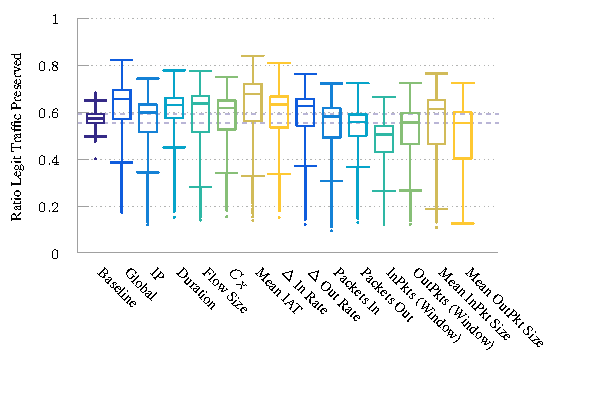
\includegraphics[width=0.9\linewidth]{../plots/ftprep-cap-box}
	\vspace{-1cm}
	\caption{
		Learned performance of Instant Control agents when benign traffic is UDP-like, using only a single feature as a basis for decisions.
		Mean IAT, inbound packet sizes, and global state offer the best predictive performance, while most features offer marginal advantage over the unprotected baseline.
		\label{fig:udp-feature-plots}
	}
\end{figure}

%\begin{figure}
%	\centering
%	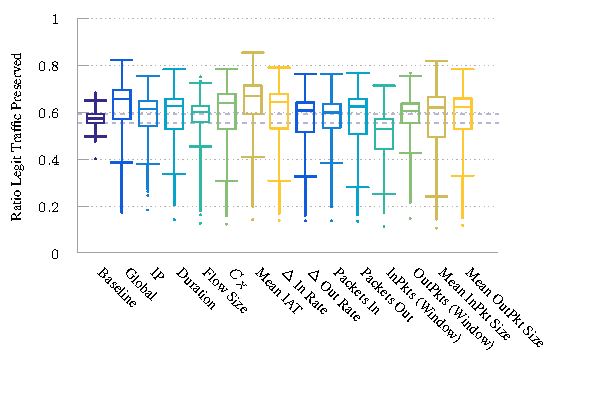
\includegraphics[width=\linewidth]{../plots/ftprep-laf-cap-box}
%	\vspace{-1.2cm}
%	\caption{
%		?? UDP, combined with last action.
%		\label{fig:udp-laf-feature-plots}
%	}
%\end{figure}

\begin{figure}
	\centering
	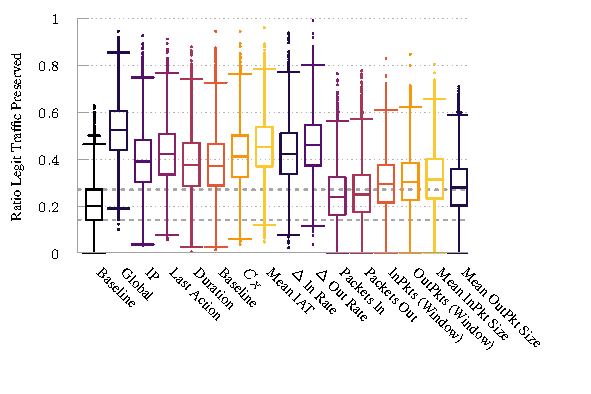
\includegraphics[width=0.9\linewidth]{../plots/ftprep-tcp-cap-box}
	\vspace{-1cm}
	\caption{
		Learned performance of Instant Control agents when benign traffic is TCP-like, using only a single feature as a basis for decisions.
		All of the chosen features can offer a marked improvement over no protection at all.
		Global state and Mean IAT still offer the greatest improvement above baseline, but packet-level statistics are considerably less effective for this class of traffic.
		\label{fig:tcp-cap-feature-plots}
	}
\end{figure}

\begin{figure}
	\centering
	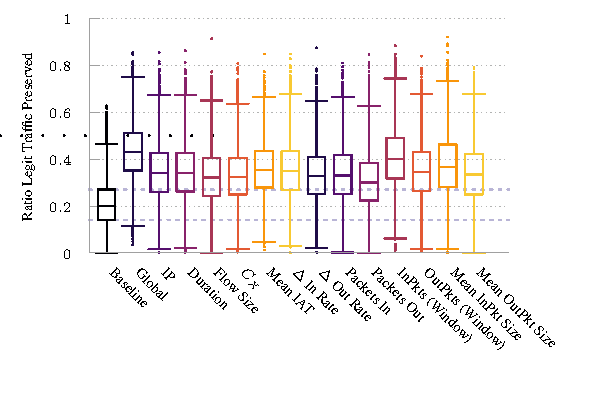
\includegraphics[width=0.9\linewidth]{../plots/ftprep-tcp-laf-cap-box}
	\vspace{-1cm}
	\caption{
		Learned performance of Instant Control agents when benign traffic is TCP-like, combining each feature with the last action taken as a basis for decisions.
		This combination causes a significant improvement in the effectiveness of packet-level and per-window statistics.
		\label{fig:tcp-laf-feature-plots}
	}
\end{figure}

The main element required to move to a per-source model is a feature set which offers high predictive power, such that behavioural differences are readily apparent to an agent.
Elaborating further on the statistics discussed in \cref{sec:motivation} which others have shown to be effective, we believe the following features to be useful (and humanly justifiable), and offer an investigation into their use alongside different traffic types:
%?? We use these features, and why...

\fakepara{Global state}
This is the vector of current load measurements along a flow's path introduced in \cref{sec:feature-space}.
These values indicate the overall health of the network, and crucially are all measurements which an agent directly controls.

\fakepara{Source IP address}
While ordinarily trivial to spoof (and thus of limited use for many classes of attack), reflectors are themselves legitimate services being abused by spoofing attackers.
As a result, they communicate with attack victims using their own IP address.
In real-world scenarios the addresses of a set of reflector nodes might exhibit similarity (such as the same CIDR block) due to network uncleanliness \cite{DBLP:conf/imc/CollinsSFJWSK07}, e.g., similarly unhardened services exposed by a single organisation.

\fakepara{Last action taken}
This encodes an agent's current belief in the maliciousness of a flow.
This feature also potentially allows forgiveness, serving as a reference point for determining whether a source mistakenly marked as malicious exhibits different falloff behaviour after punishment.
It's important to note that this feature only makes sense once combined with another flow feature, and never appears individually tile-coded.

\fakepara{Flow duration and size}
Features which describe the length of time a connection has been active, and the amount of data transferred within that time.
An extraordinarily long flow, having sent a lot of data, could be more likely to be an amplifier: though most (\SI{62}{\percent}) waves of amplifier traffic last shorter than \SI{15}{\minute} \cite{DBLP:conf/raid/KramerKMNKYR15}, this is considerably longer than the typical length of an HTTP request/response.

\fakepara{Correspondence ratio}
The ratio between upstream and downstream traffic for a source IP.
We define this to be $C_X = \min(\uload{\cdot}, \dload{\cdot})/\max(\uload{\cdot}, \dload{\cdot})$, where a value close to 0 indicates strong asymmetry.

\fakepara{$\mathbf{\Delta}$ Send/receive rate}
The change in traffic rates caused by the last action.
Behavioural changes induced by bandwidth expansion/reduction are expected to be most visible in these fields.

\fakepara{Mean inter-arrival time (IAT)}
A measure of how often packets arrive at the agent's parent switch; low IATs indicate a high number of packets per second, and can be a possible marker of malicious behaviour.
We only make use of the mean IAT of \emph{inbound} traffic.

\fakepara{(Per-window) packet count}
The amount of packets sent to/from a source over a flow's lifetime (or the current window of measurement), similar in use to flow size and mean IAT.

\fakepara{Mean packet size per window}
Legitimate flows, both TCP- and UDP-based, often transmit packets with a distribution of sizes.
Attack traffic is not likely to be so diverse: we might expect solely max-size packets in the case of amplification attacks, or minimum-size packets in other classes of flooding attack.

The exclusion of features such as source/destination ports or protocol numbers is a deliberate choice.
If \emph{QUIC} (or a similar protocol) were to become ubiquitous, then these fields would have little to no correlation with the class of traffic a flow might contain.
Our aim was to design around this constraint as a form of future-proofing.

\begin{table}
	\centering
	\caption{Tile coding windows for each feature.\label{tab:codings}}
	
	\begin{tabular}{@{}ll@{}}
		\toprule
		New Feature (unit) & Range \\
		\midrule
		Load (\si{\mega\bit\per\second}) & $[0, U_s]$ \\
		IP & $[0, 2^{32}-1]$ \\
		Last Action (\si{\percent}) & $[0, 1]$ \\
		Duration (\si{\milli\second}) & $[0, \num{2000}]$ \\
		Size (\si{\mebi\byte}) & $[0,10]$ \\
		Correspondence Ratio & $[0,1]$ \\
		Mean IAT (\si{\milli\second}) & $[0, \num{10000}]$ \\
		$\Delta$In/Out Rate (\si{\mega\bit\per\second}) & $[-50, 50]$ \\
		Packets In/Out & $[0, 7000]$ \\
		Packets In/Out Window & $[0, 2000]$ \\
		Mean In/Out Packet Size (\si{\byte}) & $[0, 1560]$ \\
		\bottomrule
	\end{tabular}
\end{table}

All of the above features, save for global state, are 1-dimensional.
\Cref{fig:udp-feature-plots} shows the effectiveness of each feature for UDP (resp.\ \cref{fig:tcp-cap-feature-plots} for TCP), using a single-destination topology (\cref{sec:single-dest}) with $n=2$ hosts per egress point averaged over 10 episodes.
\Cref{fig:tcp-laf-feature-plots} demonstrates how feature accuracy varies when tiled alongside \emph{last action}, with similar trends being observed when the same technique is applied with UDP traffic (omitted).
%?? Core findings---different protocols need different features, so everything we proposed above has a use!
The plots demonstrate that different protocols and traffic classes are best defended by different features---as such, every feature presented has value in a complete model.
All features converge to their highest-observed performance within around \num{4000} timesteps.
In general, some of the most effective features are the global state, mean IAT, mean inbound packet size and $\Delta$ rates.
%?? How do they do when combined after individual training? Pretty well, especially for TCP.
%Additional testing shows that the learned per-feature policies may be easily combined (by summing action values), and that this technique is particularly effective for TCP; these results are omitted to preserve space.
%In no cases, however, do we manage to completely block attack traffic---at convergence, we observe that system load remains consistently at $U_s$.

\section{A New Normal}\label{sec:a-new-normal}

%In establishing...
%
%?? How will I structure this?
%?? Motivation -> Model -> Results?
%?? OR Use the results of the last section to springboard into here?

%From what we have seen, it is difficult (or impossible) for trace-based or numerical simulations to correctly capture certain dynamics without an extraordinary amount of care or consideration.
%As it turns out, 
%Our goal is to briefly describe an environment which tests \emph{specific} behaviours to examine the \emph{specific} problems which have arisen during our testing of past approaches.
We contribute network models built around live testing of reactive TCP and UDP traffic in an SDN-enabled environment, which is adaptable to arbitrary topologies, with an explicit focus on preserving their real-time dynamics in a way that trace-based evaluation cannot.
First and foremost, we are interested in representative load and packet inter-arrival characteristics and in how these characteristics evolve in response to actions.
We introduce these models because we are interested in capturing interactive, correlated back-and-forth exchanges associated with live HTTP traffic; mainly because of the particular interactions between the application-level dynamics, congestion awareness at the transport level and the nature of control signal used.
%Naturally, this model is not perfect or representative for all traffic, yet it captures some of the behaviour which we expect will plague most legitimate TCP flows.
%If need be, we expect the frequency or distribution of requests could be conditioned to match observations of real-world access patterns.

%?? ANGLE: set up an environment to test \emph{specific} behaviours to examine \emph{specific} problems in past work. I make no claims that it is perfect or representative for all traffic, just for this (likely common) behaviour which I expect to plague almost all legit TCP flows.

%?? Existing sims used for testing such applications reliant on traces, or not sophisticated enough to capture interactive, back-and-forth (correlated) behaviours---possibly discarded as second-hand effects by past work when these are so crucial given user traffic patterns (and the nature of the control signal we choose to enact).

%?? Remember, the motivation is clear. We don't care so much that it is "representative" wrt a specific deployment location or network type. The whole purpose of this is that we aim to test specific behaviour which traces cannot replicate (i.e., correlated back-and-forth, dynamics introduced to congestion-aware protocols, ...)
%?? If we need to, we can condition the distribution of requests according to statistics mined from an existing trace if reviewer number 2 needs that extra push to be convinced.

\subsection{Network Design}
We make use of a fully software-defined network, built using OpenFlow-aware switches in mininet alongside a controller application based on \emph{Ryu} \cite{ryu}.
All internal routers are primed with knowledge of the shortest path to each internal host, while new inbound flows register the ``way back'' for each hop used, to ensure consistent traffic conditions for each flow.
If several ports offer different (equal-length) paths to a destination, a consistent random port is chosen from the flow-hash by an OpenFlow \emph{Group action} (in \emph{select} mode).
If such information is lost, perhaps expiring due to inactivity, it suffices to forward an outbound packet on a random (outbound) port, as we assume that any external IP is reachable through any of the test network's egress ports (i.e., that it is not connected to any stub autonomous systems).
The controller is also responsible for computing how switches respond to ARP requests: this need arises due to the reliance upon Linux's networking stack for live applications, and wouldn't need to be considered for purely trace-based evaluation.
%We make further use of the topology presented earlier (\cref{sec:topology}), noting that our architecture allows us to trivially extend and modify this if required.

\subsection{TCP (HTTP) Traffic Model}
%?? Legitimate traffic: TCP traffic (HTTP clients downloading web pages, dependent resources and files) with a mixture of lifetimes for each request.
To model legitimate TCP traffic, server nodes run an nginx v1.10.3 HTTP daemon, serving statically generated web pages alongside various large files and binaries.
Benign hosts run a simple libcurl-based application written in Rust, repeatedly requesting resources from the server.
Hosts and clients use the TCP Cubic \cite{rfc8312} flavour of TCP.
Each host's download rate is limited to match whatever maximum bandwidth was assigned to it, and requests several random files known to exist within a website, followed by any dependent resources for each (stylesheets, images, etc.).
On completion, a host changes its IP to generate separate statistics per-flow, while minimising downtime.
This presents a more balanced distribution of flow duration and size, with large files included to model elephant flows.

\subsection{UDP (Opus) Traffic Model}
VoIP traffic exhibits very different characteristics to the above model; packet arrivals are highly periodic due to real-time application requirements, flows have a constant bitrate, and do not react substantially to lost packets.
Interestingly, DDoS attack traffic is known to share many of these characteristics, offering an interesting detection problem.

We present a VoIP traffic model\footnote{Repository link removed for double-blind reviewing.} based on Discord\footnote{\url{https://discord.gg}}, a freely-available messaging and VoIP platform geared toward video game communities.
%We present a VoIP traffic model\footnote{\url{https://github.com/FelixMcFelix/opus-voip-traffic}} based on Discord\footnote{\url{https://discord.gg}}, a freely-available messaging and VoIP platform geared toward video game communities.
We chose Discord as our prototype due to its publicly documented API, many open source bot frameworks for experimentation, large user base, and due to the lack of models for Opus-encoded traffic.
All parameters (save for shortening of silent periods) are derived from passive measurement, API documentation, and the bot community's observations.
%?? Highly periodic, CBR

Hosts send RTP traffic with Salsa20 encrypted payloads---audio frames of length \SI{20}{\milli\second} at a target \SI{96}{\kilo\bit\per\second}.
We generate similar traffic at hosts by replaying anonymised traces gathered in general use and tabletop RPG servers; each trace contains only the size of each audio payload, entries denoting missed packets, and the duration of silent periods.
We trim these silent periods to a maximum \SI{5}{\second} due to the lengthy talk/silence bursts introduced by users in RPG servers, and estimate the size of missed packets by taking an exponentially-weighted moving average over known sizes.
Hosts punctuate audio frames with a 4-byte keepalive every \SI{5}{\second}.
All traffic passes over a central server which groups hosts into rooms, and is forwarded to other participants; we do not replicate pre-call Websocket traffic which would be used for authentication.
There is no peer-to-peer traffic---the server acts as a TURN relay \cite{rfc5766} for all hosts.
%?? Reflective factor among \emph{authenticated hosts}.

We find that each flow occupies an expected \SI{52.4}{\kilo\bit\per\second} upstream bandwidth.
To match the target upload rate assigned to each host, it runs enough individual sessions to meet the target data rate.

%?? Malicious traffic: UDP flood traffic (hping3, MTU-size packets, ). Why not min-size packets? Because the traffic generator gets in a horrible rut if I do so...
\subsection{Attack Traffic Model}
Malicious traffic is generated by use of the \emph{hping3} program, generating UDP-flood traffic targeting random ports.
Each malicious packet is MTU-sized, loosely mapping to the large frame sizes expected in an amplification attack and to ensure that emulation remains tractable.

\section{Evaluation}

%Traffic is played back from hosts via Tcpreplay at a bandwidth assigned uniformly from a `good' or `bad' distribution, each using the same pcap file with source and destination IP addresses rewritten.

We compare our work most naturally against the MARL approach introduced by \textcite{DBLP:journals/eaai/MalialisK15}, the state-of-the-art in RL-based DDoS prevention.
We are most interested in seeing how their approach contrasts with ours across different topologies and workloads.
Different network environments will also impose different levels of host density, where popular web servers may have orders of magnitude more clients than egress points from their network---we aim to see how these characteristics affect performance and learning rate.

To test this, we made use of both traffic models introduced in \cref{sec:a-new-normal} (OPUS and TCP), both topologies discussed below (1-dest vs Fat-Tree), and vary the amount of hosts typically communicating over each agent's ingress/egress node.
Additionally, we evaluated our new models in multi-agent mode (\emph{separate}, no model sharing), and in single-agent mode (\emph{single}, 0-cost perfect information sharing).
In each case, the algorithm's performance was averaged over \num{10} episodes of length \num{10000} timesteps (setting each agent's $\wvec{}=\bm{0}$ between episodes).
Host allocations at the beginning of each episode were generated pseudorandomly to ensure fairness between episodes.

All experiments were executed on Ubuntu 18.04.2 LTS (GNU/Linux 4.4.3-040403-generic x86\_64), using a 4-core Intel Core i7-6700K (clocked at \SI{4.2}{\giga\hertz}) and \SI{32}{\gibi\byte} of RAM.
%All code underpinning these findings is available on a public repository\footnote{\url{https://github.com/FelixMcFelix/rln-dc-ddos-paper}}.
%All code underpinning these findings is available on a public repository.\footnote{Private until publication.}

\subsection{Single Destination}\label{sec:single-dest}
%?? Move description of tree topol to here.
The network is tree-structured, where one server $s$ connects through a dedicated switch to $k$ team leader switches, each connected to $\ell$ intermediate switches, which in turn each connect to $m$ egress switches.
We then have $N_{\mathit{hosts}} = k \ell m n$.
\Cref{fig:marl-topol} demonstrates this visually.

%Although \citeauthor{DBLP:journals/ccr/MahajanBFIPS02a}, the originators of this topology, make it clear that it exists as a fairly unrepresentative example \cite{DBLP:journals/ccr/MahajanBFIPS02a}, it remains the case that such a network topology allows for functional testing, and indeed is illustrative of one way in which attack traffic might aggregate in the network.
%It is hard, however, to argue its relevance to specific classes of victim or to reason about the interactions it might have with dependent applications.
%We aim to address this through \cref{sec:performance-in-an-emulated-environment}.

To test this, we configured the network topology using $k=2$ teams, $\ell=3$ intermediate nodes per team, $m=2$ agents per intermediate node, and $n \in \{2, 4, 8, 16\}$ hosts per learner.
This is a slight simplification of the \textquote{online} experiment as presented by \textcite{DBLP:journals/eaai/MalialisK15}, choosing fewer teams but remaining as a single server with a fan-out network.
%The algorithm parameters were set at $\gamma=0$ (leading to opportunistic behaviour), $\alpha=0.05$, having linearly annealed $\epsilon=0.2 \rightarrow 0$ by $t=3000$.
%Benign and malicious hosts uploaded between \SIrange{0}{1}{\mega\bit\per\second} and \SIrange{2.5}{6}{\mega\bit\per\second} respectively, and hosts were redrawn at each episode's start with $\operatorname{P}(\mathit{malicious})=0.4$.
%$U_s$ was fixed at $k \ell mn+2$ \si{\mega\bit\per\second}.
%The performance of each choice of $n$ was averaged over \num{10} episodes of length \num{10000} timesteps (setting each agent's $\wvec{}=\bm{0}$ between episodes).
%Host allocations were generated pseudorandomly to ensure fairness between choices of $n$.
%These parameter choices match those of the original study to enable direct comparison, and are (to the best of our knowledge) arbitrary, but we justify our range of $n$ as capturing increasing scales of host activity.

\begin{figure}
	\centering
	\resizebox{0.8\linewidth}{!}{
		\begin{tikzpicture}[
		texts/.style = {text=black},
		labeltexts/.style = {text=uofgsandstone},
		treeline/.style = {draw=uofgburgundy},
		treenode/.style = {texts, circle, centered, fill=white, treeline},
		load/.style = {fill=uofgcobalt},
		loadhide/.style = {fill=uofgcobalt!40!white},
		external/.style = {fill=uofgrust},
		externalhide/.style = {fill=uofgrust!40!white},
		hideline/.style = {draw=uofgsandstone!40!white},
		hidenode/.style = {treenode, hideline},
		grow'=right
		]
		\node[treenode, label={[texts]above:Server}] (root) {}
		child [treeline] { node [treenode, label={[texts]above:Core}] (sswitch) {}
			child [treeline] { node [treenode, label={[texts]above:Leader}] (teaml) {} 
				child [treeline] { node [treenode, label={[texts]above:Intermediate}] (inter) {}
					child [treeline] { node [treenode, load, label={[texts]above:Agent/Egress}] (agent) {}
						child [treeline] { node [treenode, external] (extern) {}
							child [treeline] { node [treenode, external, label={[texts]above:Host}] (host) {} }
							child [hideline] { node [hidenode, externalhide] (endhost) {} }
						}
					}
					child [hideline] { node [hidenode, loadhide] (endagent) {} }
				}
				child [hideline] { node [hidenode] (endinter) {} }
			}
			child [hideline] { node [hidenode] (endteaml) {} }
			edge from parent
			node[below, labeltexts] {$U_s$}
		};
		
		%\draw[-] (teaml) -- (endteaml);
		\node [labeltexts] (kdots) at ($(teaml)!0.5!(endteaml)$) {$\rvdots$};
		\node [labeltexts, right = -0.1cm of kdots] {$k$};
		\node [labeltexts] (ldots) at ($(inter)!0.5!(endinter)$) {$\rvdots$};
		\node [labeltexts, right = -0.1cm of ldots] {$\ell$};
		\node [labeltexts] (mdots) at ($(agent)!0.5!(endagent)$) {$\rvdots$};
		\node [labeltexts, right = -0.1cm of mdots] {$m$};
		\node [labeltexts] (ndots) at ($(host)!0.5!(endhost)$) {$\rvdots$};
		\node [labeltexts, right = -0.1cm of ndots] {$n$};
		\end{tikzpicture}
	}
	\caption{
		Network topology diagram, showing how the server and its core switch's $k$ teams are structured, with $\ell$ intermediate routers per team, connected to $m$ agents which each moderate $n$ hosts beyond a single external switch.
		%	Empty nodes are considered to be internal.
		Red nodes are external, and each blue node hosts an agent.
		\label{fig:marl-topol}
	}
\end{figure}

\subsection{Multiple Destinations}
The previous topology allows for direct comparison against the state-of-the-art, and indeed is illustrative of one way in which attack traffic might aggregate in the network.
It is hard, however, to argue its relevance to specific classes of victim or to reason about the interactions it might have with dependent applications.
In contrast, the fat-tree topology \cite{DBLP:conf/sigcomm/Al-FaresLV08} sees regular use in real-world datacentres and scales well horizontally.

%?? Come up with description of fat-tree (multi-dest) topol.
%?? Why fat tree? regularly appears in modern datacentres.
%?? $k=4$ fat-tree , with one pod hosting two servers $s_0,s_1$.
We use a $k=4$ fat-tree, with one pod hosting two servers $s_0$ and $s_1$.
$n$ external hosts connect through each core switch (where agents are hosted), and communicate with $s_0, s_1$ uniformly randomly.
Both servers host identical services.
We set $n \in \{6, 12, 24, 48\}$ hosts per learner (keeping $N_{\mathit{hosts}}$ identical to each tier of the single-host topology), and restrict $U_{s_0} = U_{s_1} = U_s / 2$.

\subsection{Parameters}
The algorithm parameters were set at $\alpha=0.05$, linearly annealing $\epsilon=0.2 \rightarrow 0$ by $t=3000$ in the case of Marl (\num{8000} actions per agent in the \emph{Instant/Guarded} models).

Benign hosts uploaded between \SIrange{0}{1}{\mega\bit\per\second}, and hosts were redrawn at each episode's start with $\operatorname{P}(\mathit{malicious})=0.4$.
%The original introduction of this approach to direct-control reinforcement learning as introduced by \textcite{DBLP:journals/eaai/MalialisK15} fails to consider key cases: the absence of a suitable heuristic classifier $g(\cdot)$, disjoint ranges of traffic distribution (i.e., the presence of benign heavy-hitters), the accurate simulation of TCP-like behaviour (and its effects on collateral damage), and high densities of hosts at egress points.
%?? Why? ...
%Of these, the latter two are most deserving of a closer investigation, as they have stronger implications for wide-scale deployment.
%These are important issues, particularly when we consider real-world deployment.
%Heuristic estimates of traffic legitimacy come with computational cost and couple the reward function to the accuracy of the estimator, hosts often show diversity in their own traffic patterns (perhaps being multi-modal), and it is known that TCP is the most used transport protocol for Internet traffic \cite{DBLP:conf/saint/ZhangDJC09}.
%?? NEED TO VERIFY VOLUME OF CONGESTION-AWARE PROTOCOLS
Malicious hosts sent \SIrange{2.5}{6}{\mega\bit\per\second} when attacking UDP traffic, though when using TCP-like traffic, each attacker's upload range had to be increased to \SIrange{4}{7}{\mega\bit\per\second} to meaningfully impact benign flows.
Given $n$ and $\operatorname{P}(\mathit{malicious})$, we see an expected malicious bandwidth \numrange{1.27}{1.87} and \SIrange{2.03}{2.18}{$\! \times U_s$} respectively.
%The expected fraction of $U_s$ consumed by each host is \SI{21.5}{\percent} for $n=2$, and \SI{2.84}{\percent} for $n=16$.

$U_s$ was fixed at $N_{\mathit{hosts}}+2$ \si{\mega\bit\per\second} (to account for burstiness), and each link had a delay of \SI{10}{\milli\second}.
All links had unbounded capacity, save for server-switch connections.
These parameter choices match those of the original study to enable direct comparison, and many are (to the best of our knowledge) arbitrary, but we justify our range of $n$ as capturing increasing scales of host activity.

\section{Results}
\label{sec:the-results-of-doing-so}

We now examine the performance of our two new models (\emph{Instant}, \emph{Guarded}) as compared against existing RL work (\emph{Marl}) under different traffic behaviour and topologies, varying the host-to-learner ratio $n$ and environment.
%?? Probably best just to look at top level stuff, and THEN a simplified comparison for each intended improvement (like banded rewards).
%Additionally, we examine the performance effects of environmental characteristics and potential improvements: negative reinforcement, the case where one agent makes all decisions, and pre-training on individual features.
We present the average rewards for all combinations of these factors in \crefrange{tab:av-vals}{tab:av-ecmp-vals}---these provide a rough idea of expected performance, giving the highest-performing model in bold.
Average rewards take into account any portions of time that an agent allows illegal system states.
Several plots augment this, illustrating peak performance or the amount of time which an agent requires to learn.

\begin{table}
	\centering
	\caption{Average reward for combinations of model, host density and traffic class with a single destination.\label{tab:av-vals}}
	
	\resizebox{\linewidth}{!}{
		\expandableinput ../tables/infocom-tree-avg-reward.tex
	}
\end{table}
\begin{table}
	\centering
	\caption{Average reward for combinations of model, host density and traffic class with multiple destinations.\label{tab:av-ecmp-vals}}
	
	\resizebox{\linewidth}{!}{
		\expandableinput ../tables/infocom-ecmp-avg-reward.tex
	}
\end{table}

\subsection{Congestion-unaware traffic}
%\begin{figure}
%	\centering
%	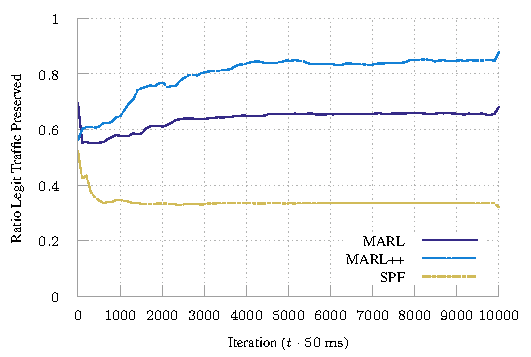
\includegraphics[width=0.9\linewidth]{../plots/udp-2}
%	
%	\caption{
%		Online performance for $n=2$ hosts per egress point when benign traffic is UDP-like.
%		Although Marl++ offers a marked improvement (a peak $\sim$\SI{30}{\percent} more benign traffic arrives unimpeded), SPF significantly underperforms for this relatively simple topology.
%		Non-SPF agents start off reasonably well, slowly learning better policies.
%		\label{fig:udp-2}
%	}
%\end{figure}
%\begin{figure}
%	\centering
%	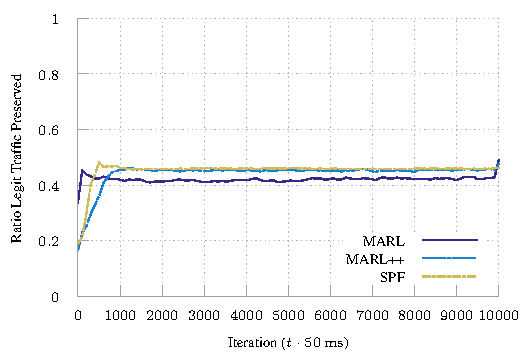
\includegraphics[width=0.9\linewidth]{../plots/udp-16}
%	
%	\caption{
%		Online performance for $n=16$ hosts per egress point when benign traffic is UDP-like.
%		Marl++ remains marginally ahead of its predecessor, though both have undergone a significant drop in effectiveness.
%		SPF, remarkably, displays performance on par with Marl++ for this more difficult topology.
%		Both of the new models take longer to train, but achieve better peak and average performance than Marl.
%		\label{fig:udp-16}
%	}
%\end{figure}
\begin{figure}
	\centering
	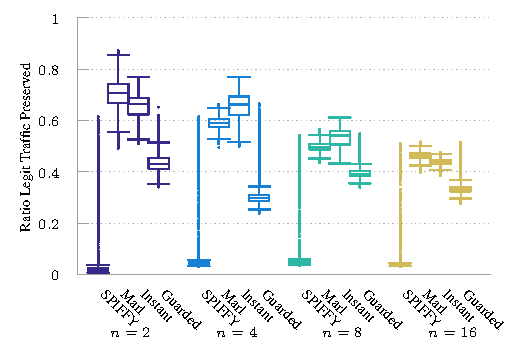
\includegraphics[width=0.95\linewidth]{../plots/tnsm-udp-box-separate}
	
	\caption{
		Online performance for Opus benign traffic in a single-destination network, multi-agent mode.
%		Marl++ offers a marked improvement (a peak $\sim$\SI{30}{\percent} more benign traffic arrives unimpeded) at small $n$, and remains marginally ahead of its predecessor by $n=16$, though both have undergone a significant drop in effectiveness.
		\emph{Instant} outperforms Marl for $n \in \{4, 8\}$ (with higher variance), but performs similarly to Marl at $n\in \{2, 16\}$.
		\emph{Guarded} always underperforms compared to the other agent designs in this problem variant.
%		SPF, remarkably, slightly outperforms Marl++ (with lower variance) for this more difficult topology despite being worse for smaller $n$.
%		Both of the new models take longer to train, but achieve better peak and average performance than Marl.
%		?? REWORK/MAKE ACCURATE
		\label{fig:udp-tree-box}
	}
\end{figure}

%\begin{figure}
%	\centering
%	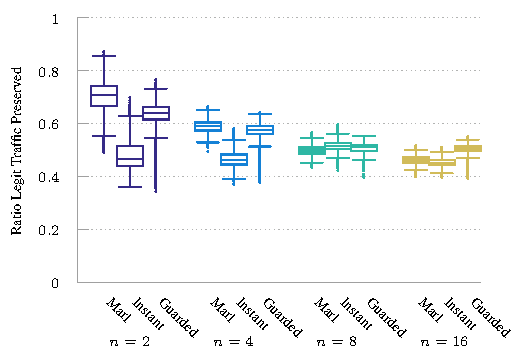
\includegraphics[width=0.95\linewidth]{../plots/tnsm-udp-box-single}
%	
%	\caption{
%		Online performance for Opus benign traffic in a single-destination network, single-agent mode.
%		?? DO I need this?
%		\label{fig:udp-tree-box-single}
%	}
%\end{figure}
%
%\begin{figure}
%	\centering
%	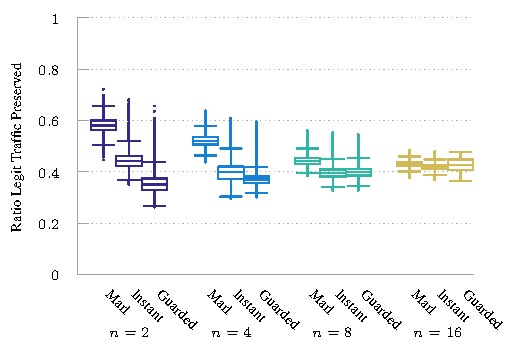
\includegraphics[width=0.95\linewidth]{../plots/tnsm-ecmp-udp-box-separate}
%	
%	\caption{
%		Online performance for Opus benign traffic in a multi-destination network, multi-agent mode.
%		?? DO I need this?
%		\label{fig:udp-ecmp-box}
%	}
%\end{figure}
%
%\begin{figure}
%	\centering
%	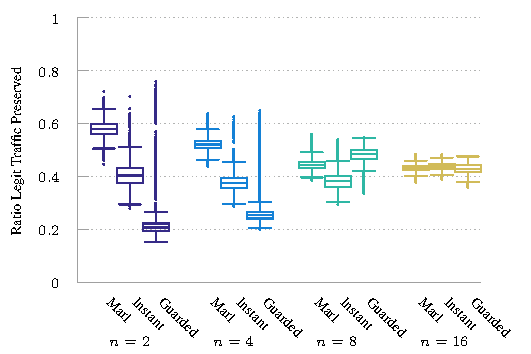
\includegraphics[width=0.95\linewidth]{../plots/tnsm-ecmp-udp-box-single}
%	
%	\caption{
%		Online performance for Opus benign traffic in a multi-destination network, single-agent mode.
%		?? DO I need this?
%		\label{fig:udp-ecmp-box-single}
%	}
%\end{figure}

In a single-destination network, we observe that Marl's performance degrades as $n$ increases.
Typically, our \emph{Instant} agent design achieves the best performance in multi-agent mode, reducing collateral damage above the current state-of-the-art, but sharply degrades at low $n$ when agents share experience.
We see a reversal of this trend for the \emph{Guarded} model, which improves as $n$ increases and in single-agent mode---when $n\ge4$, the single-agent variant offers consistent improvement.
%Across all choices of $n$, we see that Marl++ exhibits reduced collateral damage compared to Marl, with SPF starting poorly yet becoming more effective for larger $n$ (\cref{tab:av-vals}, \emph{Capped}, UDP).
\Cref{fig:udp-tree-box} shows the preserved traffic in multi-agent mode.

%?? Discuss multi-dest topol once all results available.
When defending multiple destinations, we see a sharp decrease in the effectiveness of all agent designs.
Our \emph{Instant} and \emph{Guarded} designs become more effective as $n$ increases, while Marl's effectiveness is roughly constant (aside from the outlier at $n=12$).

\subsection{Congestion-aware traffic}
%\begin{figure}
%	\centering
%	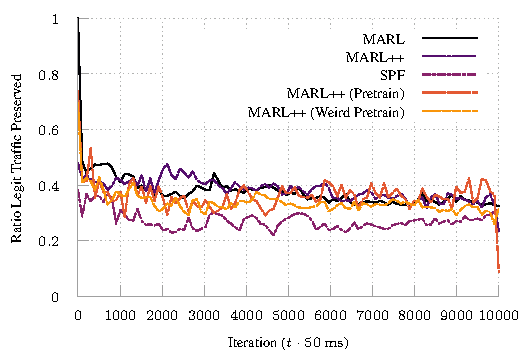
\includegraphics[width=0.9\linewidth]{../plots/tcp-2}
%	
%	\caption{
%		Online performance for $n=2$ hosts per egress point when benign traffic is TCP-like.
%		Marl++ and Marl achieve very similar performance, starting off similarly well without notable improvement over an episode.
%		SPF's performance is disappointingly close to baseline, indicating that it is as useful as having no defence system.
%		\label{fig:tcp-2}
%	}
%\end{figure}
\begin{figure}
	\centering
	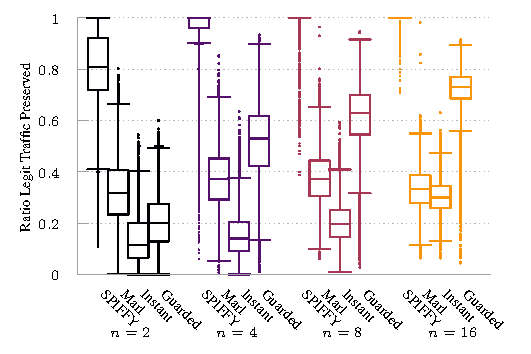
\includegraphics[width=0.95\linewidth]{../plots/tnsm-tcp-box-single}
	
	\caption{
		Online performance for HTTP benign traffic in a single-destination network, single-agent mode.
		\emph{Instant} and \emph{Guarded} exhibit essentially identical efficacy at $n~=~2$, protecting less traffic than Marl.
		Only \emph{Guarded}'s performance rapidly increases with $n$, achieving considerably better median performance and lower variance than the other models.
		The longer tails of outliers typically indicate the longer training time the new models require---we observe that \emph{Guarded} typically has considerably lower variance once it has converged on a stable policy.
		\label{fig:tcp-tree-box}
	}
\end{figure}
%\begin{figure}
%	\centering
%	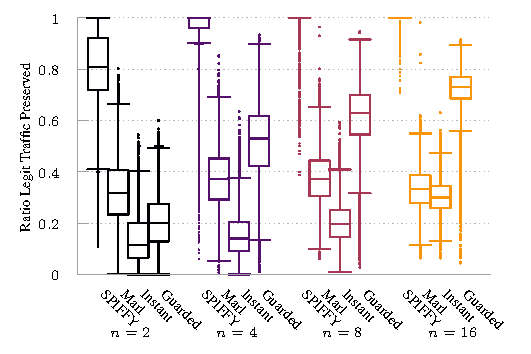
\includegraphics[width=0.95\linewidth]{../plots/tnsm-tcp-box-single}
%	
%	\caption{
%		Online performance for HTTP benign traffic in a single-destination network, single-agent mode.
%		?? DO I need this?
%		\label{fig-tcp-tree-box-single}
%	}
%\end{figure}
\begin{figure}
	\centering
	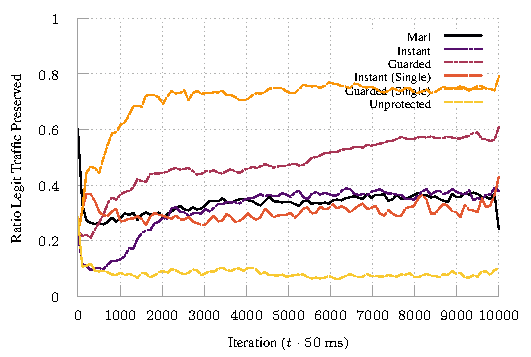
\includegraphics[width=0.95\linewidth]{../plots/tnsm-tcp-16-single}
	
	\caption{
		Online performance of standard and single-agent models in a single-destination network with $n=16$ hosts per egress point and HTTP benign traffic.
		At this level of host density, \emph{Guarded} reaches higher peak performance sooner and is considerably more consistent throughout the episode.
		\emph{Guarded} benefits greatly from information sharing, converging to protect around \SI{75}{\percent} of TCP traffic within \SI{100}{\second}.
		The \emph{Instant} model converges to Marl's level of performance.
%		With a single agent, Marl++ shows worse performance, while SPF improves significantly and continues to learn well past annealing $\epsilon \rightarrow 0$.
		\label{fig:tcp-tree-16}
	}
\end{figure}

%\begin{figure}
%	\centering
%	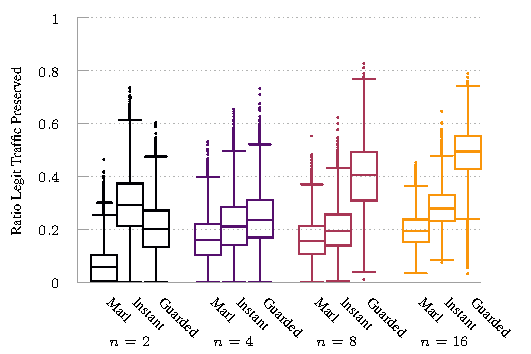
\includegraphics[width=0.95\linewidth]{../plots/tnsm-ecmp-tcp-box-separate}
%	
%	\caption{
%		Online performance for HTTP benign traffic in a multi-destination network, multi-agent mode.
%		?? DO I need this?
%		\label{fig:tcp-ecmp-box}
%	}
%\end{figure}

%\begin{figure}
%	\centering
%	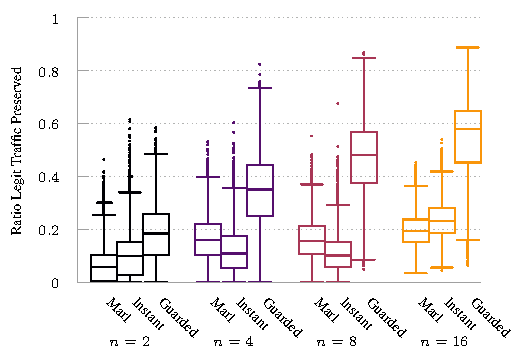
\includegraphics[width=0.95\linewidth]{../plots/tnsm-ecmp-tcp-box-single}
%	
%	\caption{
%		Online performance for HTTP benign traffic in a multi-destination network, single-agent mode.
%		?? DO I need this?
%		\label{fig:tcp-ecmp-box-single}
%	}
%\end{figure}

%\begin{figure}
%	\centering
%	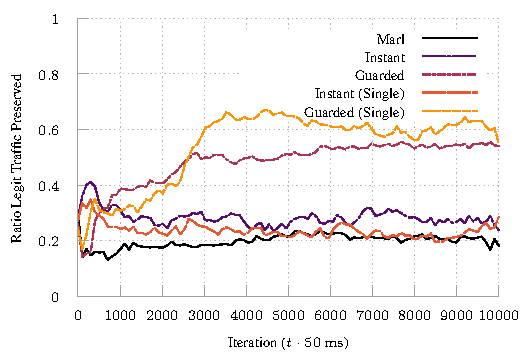
\includegraphics[width=0.95\linewidth]{../plots/tnsm-ecmp-tcp-16-single}
%	
%	\caption{
%		?? Eh
%		\label{fig:tcp-ecmp-16}
%	}
%\end{figure}

\Cref{tab:av-vals} shows that Marl offers a low (though fairly consistent) level of protection for TCP traffic, which the \emph{Instant} agent offers no substantial improvement over.
However, \emph{Guarded} agents offer a remarkable improvement for this class of traffic, particularly when experience can be shared---offering a \SI{2.21}{$\!\times$} improvement over the state-of-the art during training, which is made clearer in \cref{fig:tcp-tree-box}.
\Cref{fig:tcp-tree-16} shows that this model can protect a peak \SI{80}{\percent} of TCP traffic (\SI{2.5}{$\!\times$} improvement over Marl, \SI{8}{$\!\times$} more traffic than no defence system) after just \SI{100}{\second}, but also that all of the new models require considerably longer than Marl to learn their best-achieving policy.
%SPF reaches a stronger plateau before \emph{both}, remaining more consistent and appearing to continue learning.

%?? Discuss multi-dest topol once results available.
We observe that the same trends present themselves in the multi-destination topology: \emph{Guarded} remains the best fit for TCP, in both training modes.
Crucially, the rigid tree of learners and teams which define Marl, along with its lack of action granularity, seem to be a poor fit in this environment.

%\subsection{Single-agent performance}
%Making all decisions with a single agent is roughly equivalent to having a zero-cost communication channel between each pair of agents, theoretically allowing faster training by giving each agent more experience.
%Curiously, we observe that this often leads to drastically worse policies when used as part of Marl++ for small $n$, but makes SPF a considerably more competitive model---especially for TCP, and as $n$ grows larger (\cref{fig:tcp-16}).
%Single-agent SPF almost consistently outperforms Marl.
%We discuss our conjectures for why this reversal occurs in \cref{sec:discussion}.

\subsection{Computational Cost}
%?? Consider talking about the execution times of the old MARL approach here? They're real nice (as expected), so we have lots of room to play around with while (hopefully) remaining under the 1ms target time given by \textcite{DBLP:conf/sigcomm/ChenL0L18}.

%Overall, each episode takes around \SI{10}{\minute} to run, while each set of \num{10} requires around \SI{2}{\hour} due to additional set-up/tear-down costs associated with mininet.
Measurements taken during each of these experiments indicated that the cost of computing any action is typically within \SIrange{80}{100}{\micro\second}.
This is reassuring when measured alongside the insights from other work, since as we discussed in \cref{sec:systems-considerations} the python language bottlenecks performance.
\Textcite{DBLP:conf/sigcomm/ChenL0L18} observe that, ideally, actions must be computed and taken within \SI{1}{\milli\second} to have a meaningful affect on short flows.
%Most flows are short, and flow-size follows a heavy-tailed distribution.
That our starting point falls significantly below this threshold allows us to safely consider more costly actions or larger state spaces, which would typically increase the computational cost.
%?? TODO: update with modern numbers...

\section{Discussion}\label{sec:discussion}

%?? New angle -- \emph{Guarded} offers substantal improvements for \emph{most} internet traffic according to the stats we know. Is accurate protection of beningn UDP traffic actually more difficult?

%Talk about flaws here, what could go wrong...

%?? Why does SPF only do well sometimes? Model is actually more difficult to learn, so it seems to do best when it has a larger set of decisions to learn from. But, it does worse for TCP?
\fakepara{Model performance}
Of the results presented, \emph{Guarded}'s unpredictable (often worse) starting performance is unexpected, given its far smaller action space.
It's natural to expect that this would make the model easier to learn, but the additional state required appears to make the task \emph{harder}, beyond even the value of choosing a non-zero discount factor (adding forward-planning to explicitly mitigate this effect).
Accordingly, we see that this design performs best (and exhibits considerably lower variance) when agents learn from as much knowledge as possible: high $n$ and single-agent training.
To filter incoming traffic from a source, it must decide to degrade their inbound traffic multiple times in a row, reducing the likelihood that a legitimate flow is punished by accident.
Our belief is that \emph{Guarded} is a considerably stronger model for these reasons, and its successes offer strong rationale to consider the best schemes for efficient information sharing.
Paradoxically, \emph{Instant} generally achieves the best performance for UDP traffic yet actively suffers when trained as a single learner---this may occur due to a roughly even spread of values between disparate actions, due to shared characteristics between legitimate and malicious flows.

%?? May be hard to learn multiple features at once while controlling multiple flows while contending with many more agents, with harder dynamics like TCP. Does this hinder learning in the long run?
Although we have improved upon Marl in both identified problem cases, the improvements are not quite on the order we'd expect in the case of UDP traffic.
%?? I don’t know if you want to also mention the problem of things getting “stuck” in locally optimal (but globally sub-optimal) policies. I think it’s fairly uncontroversial that an increase in state space would make this more likely. Also, the lack of discounting could play a large role (and more so as the state space becomes more complex…
The most likely explanation is that agents are converging to, and becoming stuck in, locally optimal (but globally sub-optimal) policies.
The increased state space size makes this a more likely occurrence, as is the unclear affect of hyperparameters ($\alpha$, $\gamma$) as we scale up the state space.
We suspect that these difficulties may be exacerbated by the competitive nature of learning that these models embody: agents are learning action values for multiple features simultaneously, taking many actions at once (making it harder to observe the true value of each action), and controlling shared global state.
Although our design does take steps to counteract such effects, these mitigations may not be enough.
Moreover, benign UDP traffic shares many characteristics with attack traffic, suggesting that more training samples or some unknown feature might aid control, or that it may be worthwhile to extensively pre-train agents non-competitively on each feature using individual flows.

%It is likely that the design of Marl++ 
%?? Need to mention that Marl performs lower than their paper's numbers for TCP...

%Finally, it is crucial to note that the models and techniques presented here are an improvement , this work still trails behind existing (exact) DDoS flow detection mechanisms.
Most importantly, what we wish to impart is the knowledge that while the models and techniques we present here are a significant improvement over past RL-based work, this work still trails behind existing (exact) DDoS flow detection mechanisms.
Although we have conducted work to map the territory to some extent, there are still more advancements to be made before RL-based DDoS defence is truly competitive.
The benefits we have at present are, however, substantial.
What we offer above the alternate approaches we discuss in \cref{sec:related-work} are potentially more flexible deployments and low-overhead decision-making, without requiring active measurement or the network resources and capabilities that the most effective techniques rely upon.
The techniques we propose offer substantial improvements for the defence of congestion-aware traffic, which remains the most prevalent class of traffic on the internet today.
Moreover, our decision making processes are entirely agnostic of the protocol or content of inbound traffic, offering future-proofing against the introduction of new transports.

\fakepara{Security concerns and vulnerability}
Can an agent be flooded with new flows to reduce their ability to make decisions?
One of the risks introduced by our timed random sequential policy updates is that so much work can be queued up that an agent is never able to act on some attack flows.
The natural solution is to impose an upper bound on the amount of action computations/policy updates that can be performed before a work list is discarded completely.
This removes the guarantee that all flows will be visited fairly often, but if updates occur regularly then this random sampling may be sufficient to achieve good performance.

%\begin{figure}
%	\centering
%	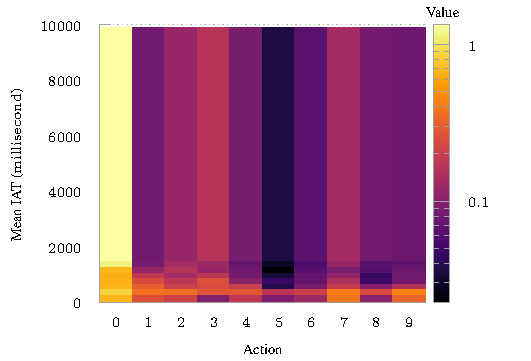
\includegraphics[width=0.9\linewidth]{../plots/policy-16-tcp-f5-mean-log}
%	
%	\caption{
%		Mean Marl action values from pre-training on mean IATs ($n=16$).
%		As these are mean values, lighter cells in each row indicate actions \emph{likely} to be taken by an agent's policy.
%		Repeated values originate from the bias tile, which is always active, and indicate regions of the state-space which have yet to be visited---here, this is most of the state space.
%		Agents visibly learn action values for tiles which override the default bias tile's preferences.
%		The measured effectiveness of this feature then suggests that a low-resolution coding over the standard region may, in fact, be a better choice.
%		We see that agents prefer to choose $p=0.0$ in most states, but higher $p$ when IATs are particularly small.
%		\label{fig:intern-16-tcp-iat}
%	}
%\end{figure}
%
%\begin{figure}
%	\centering
%	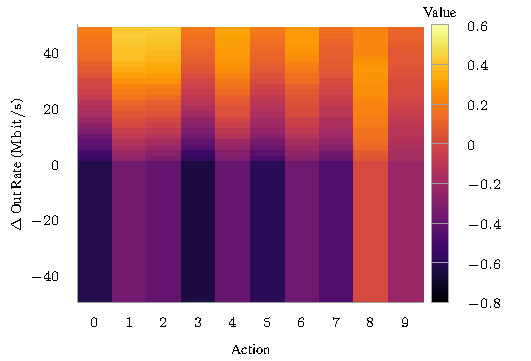
\includegraphics[width=0.9\linewidth]{../plots/policy-4-tcp-f7-mean}
%	
%	\caption{
%		Mean Marl action values from pre-training on $\Delta$ out rates ($n=4$).
%		A sudden ramp-up of server-to-host traffic is used as a strong indicator of flow legitimacy, while more punishing actions have comparatively higher value as $\Delta$ out rate decreases.
%		Furthermore, we see again that a region of the state space has gone somewhat unexplored---we observed after plotting this visualisation that many decreases in this feature are too small to hit the adjacent tile, which implies a mixed-resolution coding may improve an agent's policy further.
%		\label{fig:intern-16-tcp-something}
%	}
%\end{figure}

%?? Is the state space interpretable? Yes!
Machine learning algorithms have earned a reputation for eluding human interpretation, while being vulnerable to evasion and poisoning.
Given the risks associated with introducing such techniques in the context of security, it is natural to be concerned with the interpretability of the models we have proposed.
With the exception of global state, the tile-coding parameters we make use of ensure that the set of all outputs for each new feature we add is relatively enumerable: for $n$ tilings and $c$ tiles per dimension there are $nc^{\dim{f}}$ individual action value vectors per feature $f$ (\num{48} for the new features we introduce, \num{10368} for global state), though considerably more combinations thereof ($c^{n \cdot \dim{f}}$).
%\Cref{fig:intern-16-tcp-iat,fig:intern-16-tcp-something} show how we may visualise the portion of a policy for each feature, and describe what information can be gained from doing so.
Furthermore, system state which is dependent on many signals drawn from across a wide network (such as our global state) is difficult to exert precise control over.
These signals' topological separation, in concert with their burstiness and unpredictability, may have substantial effects on an attacker's capabilities.

\fakepara{Real-world Deployment}
Currently, we assume that switches support an extension to OpenFlow to enable remotely installable packet-drop rules, either by running a modified version of OVS on commodity hardware at these locations or through custom firmware for egress switches.
Similar functionality could be employed by making use of OpenFlow's meter rules.

Where overheads are concerned, the state space sizes guarantee that an \emph{Instant} agent's policy remains under \SI{520}{\kibi\byte}, although in practice our sparse representation typically leads to far smaller policies: $\sim$\SI{17.8}{\kibi\byte} from our experiments.
\emph{Guarded} policies are \SI{30}{\percent} of this size.
As we have described earlier, action updates require a constant number of floating point operations---\num{160} floating point additions and \num{32} multiplications per update of $\wvec{}$ with per-tile updates, above the \num{160} additions required to choose an action.
The vast majority of these operations can be vectorised trivially, if such hardware is present.
Action computation for \emph{Guarded} agents is cheaper still, requiring only \num{48} additions per action.
Beyond this, we require that egress switches are capable of co-hosting an agent (i.e., through \emph{network function virtualisation}), with the necessary hardware to support this choice.
We believe that it may be possible to implement similar behaviour on standard commodity switches through application of \emph{programmable data planes} \cite{DBLP:conf/ancs/JouetP17}.

%?? Incorrect, pickling...
%?? deployment/system guidelines, architecture, and overhead/footprint of doing this
%?? Mention: probably fewer state measurements than in our emulations, but longer measurements means less noisy (so probably more accurate)
Gathering and transmission of load/flow statistics would be difficult to perform quite as often as an emulated environment allows, without inadvertently affecting host traffic.
However, the measurements acquired in such a scenario are far more likely to be less noisy (by being collected over longer periods of time), which could aid effective training.
The main bottlenecks are most likely in forwarding the load measurements from various aggregation points (which can be made more efficient through multicast) and in running some estimator $\operatorname{g}(\cdot)$ to condition the reward function.
%?? Potential for dividing up pre-feature training across different agents, or train like this locally (sets of flows trained by 1 sub-model).
%?? Different global state per-agent? Seems this must be locally trained, just make it (everything up the chain to key destinations).
We expect that agents will be able to share policies for all features, which may help to offset the reduced rate of incoming experience.
Regardless, it will take longer to achieve enough state-state transitions to converge on a good policy.

\section{Related Work}\label{sec:related-work}

%?? Try and compare my work here when possible?

\fakepara{DDoS Prevention}
\Textcite{DBLP:conf/lcn/BragaMP10} have examined the detection of ongoing (flooding-based) DDoS attacks through \emph{self-organising maps}, making use of SDN to gather statistics effectively.
Many of their features aren't overly relevant, as their focus is not active defence or discovering \emph{which} hosts are contributing to an attack.

%?? Actually talk about Marl (???) to appease reviewer \#1.
The closest available approach within this field is that of \textcite{DBLP:journals/eaai/MalialisK15} (whom we have positioned our work against), and their contribution in applying RL to the task of intrusion prevention is significant: their work helps to show the viability of live, adaptive, feedback-loop-like control of the network to detect and prevent DDoS attacks.
They create a tree overlay topology (subdivided into teams), where each agent applies packet drop to \emph{all} flows inbound to a protected server.
%?? Recap their flaws, since they've been cut form every other aspect.
Our results show that their technique underperforms at high host density and when congestion-aware traffic dominates---that their results do not demonstrate this suggests an evaluation driven purely by traces (rather than live application dynamics).

\emph{SPIFFY} \cite{DBLP:conf/ndss/KangGS16} aims to remedy transit-link attacks by observing how flows from each source respond to a sudden increase in available bandwidth.
\Citeauthor{DBLP:conf/ndss/KangGS16} realise that bots participating in an attack are often unable to match this bandwidth expansion due to having already saturated the capacity of their outbound links, while legitimate flows typically speed up to match the new fair-share rate.
%Attackers must either be detected or reduce the throughput of each bot, increasing the cost of launching an attack.
Unlike our approach (and due to the class of attacks it is designed to defend against), SPIFFY is intended to be deployed within ASes, although some of our feature choices are backed by similar observations.
A weakness of their approach is that computing a route to measure bandwidth expansion on real networks can be costly (up to \SI{14}{\second} for the Cogent topology), and that the low expansion factors in real network can require more ``rounds'' of filtering. 
Their assumptions about traffic response to such bandwidth expansion may not extend to HTTP DASH traffic or constant bitrate traffic (e.g., UDP VoIP traffic), both of which make up a sizeable proportion of network traffic.

\emph{Athena} \cite{DBLP:conf/dsn/LeeKSPY17} is a more generalised SDN framework for intrusion detection, but has shown the use of a \emph{k-nearest neighbours} classifier to detect individual attack flows.
Although heavyweight (and proven to be effective compared with \textcite{DBLP:conf/lcn/BragaMP10}), their comparison against SPIFFY lacks the quantitative evidence required to understand how the system compares.

\Textcite{DBLP:conf/sp/SmithS18} present techniques based on AS-level routing to tackle both transit-link and flooding-based attacks.
This view is taken due to the perceived cost of per-stream classification and inherent sensitivity to adversarial examples or crafted input.
The approach is creative, relying upon BGP \emph{fraudulent route reverse poisoning} to preserve traffic to a target AS, but unlike SPIFFY the approach doesn't actually \emph{remove} the congestion.
Because of this, traditional flooding-based attacks aren't fully alleviated.

%?? Abuses of RL 
\fakepara{RL in Networks}
Earnest, well-considered application of RL towards the challenge of intrusion detection/prevention has seen comparatively little examination.
Past work exhibits treatment of the paradigm as a traditional classifier for anomaly detection \cite{shamshirband2014anomaly} and DDoS prevention \cite{DBLP:conf/mates/ServinK08}.
Given that one of the main strengths of RL techniques is the ability to control ongoing interaction and to adapt by observing the concrete effects of actions taken, such works don't apply the rich literature on the subject to its fullest potential.

For categorising how RL fits into solving problems, we label works as direct- or indirect-control RL.
A \emph{direct-control} RL problem is one where the RL agent(s) are learning optimal control over a set of actions to act as the \emph{primary} defence or decision-maker---requiring measurements, reward functions and action sets tailored for this purpose.
%We feel there is a shortage of work in this category at present, at least in the field of networks.
To date, the best-fitting example we have encountered is that of \textcite{DBLP:journals/eaai/MalialisK15}.

An \emph{indirect-control} RL problem is one where the role played by the agents is to act in service to \emph{another technique} responsible for decision-making, further optimising or generalising aspects of its operation beyond that of hand-coded heuristics.
A past example includes learning when best to \emph{communicate} and share knowledge between \emph{hidden Markov model} anomaly detectors \cite{DBLP:conf/paisi/XuSH07}.
%The position of this work is weakened by its reliance on the problematic `DARPA99' dataset \cite{DARPA-IDD, DBLP:conf/cisda/TavallaeeBLG09, DBLP:conf/sp/SommerP10}, but the idea itself is well-treated and this acts as a driver for improvements in this direction.
The position of this work is weakened by its reliance on the problematic `DARPA99' dataset \cite{DBLP:conf/sp/SommerP10}, but the idea itself is well-treated and this acts as a driver for improvements in this direction.
Outside of anomaly/intrusion detection, there has been growing interest in the use of reinforcement learning in data-driven networking, such as for intra-AS route optimisation \cite{DBLP:conf/hotnets/ValadarskySST17} and for resource-constrained process allocation \cite{DBLP:conf/hotnets/MaoAMK16}.
Work by \textcite{DBLP:conf/sigcomm/MaoNA17} employs client-side observations of network state and video player performance to optimise adaptive bitrate selection for multimedia streaming by RL methods.

\emph{AuTO} \cite{DBLP:conf/sigcomm/ChenL0L18} employs deep RL to perform traffic optimisation.
Crucially, they find that the vast majority of flows are short-lived, requiring effective decisions in less than a millisecond.
To overcome the high latency of action computation via a neural network, two agents are trained, handling aspects of short and long flows respectively.
The first learns to optimise the flow size thresholds which define priority allocation at each switch (and accordingly learn how best to demarcate long and short flows); these short flows are routed by ECMP.
The second agent makes bespoke decisions about routing, prioritisation etc.\ for each of the remaining long flows, who are likely to live long enough that any actions will have a significant impact.

%These works emphasise the necessity of ingenuity in effectively handling how states and actions are represented.

\section{Conclusions and Future Work}
Through this paper, we have discussed the paradigm of reinforcement learning and its relevance to network intrusion prevention.
Our belief is that the potential to learn feedback-loop-like control online and against non-stationary problems makes it particularly suited to the problems endemic to the field.

We have identified weaknesses in past approaches arising from simulation assumptions, recommending an RL agent design which acts per-flow, and have outlined the algorithmic modifications and engineering choices needed to make its deployment feasible.
Supporting this, we've presented an in-depth examination of the design of our feature space, offering quantitative and qualitative justification for our choices.
Our evaluation shows that our new agent designs considerably advance the state-of-the-art in RL-based DDoS prevention, with \emph{Guarded} agents showing the most promise for future evaluation.

The most direct improvements to be made lie in the correct protection of legitimate UDP traffic, which our agent designs have difficulty safeguarding.
Outside of this, there is scope to test these new techniques against link-flooding attacks in large-scale topologies using reward functions such as \cref{eqn:lfa-reward}.
Simulation is the most likely avenue for such evaluation.

%(rather than na\"{i}ve simulation, blind ML applications etc.) and choose well-considered pathways to solution. \emph{Call-to-action}?

%\section{Future Work}
%Airlift half of the ``conclusion'' and paste it in here, so that it can be a lot neater.
%?? Future Work? I.e., \emph{everything}: no one else is really looking at/interested in this specific kind of application of RL yet. \emph{Yet}.

%?? IDEA: try out average reward, TD($\lambda$) methods as future work...
%A natural research direction to enhance this work would be the combination of the classic function approximation techniques we make use of alongside the improved algorithms that the RL community has introduced in the past few years.
%Actor-critic methods, or algorithms based on eligibility traces are good candidates for investigation. 
The remaining weaknesses invite many further improvements worth investigation.
%?? What might we do for a reward function in the absence of heuristic estimates and/or explicit a priori knowledge? I think a good candidate is the sum of up and down throughputs (normalised by capacity sum), so long as \emph{neither exceeds the link capacity}. We can extend the team-based formulations similarly. This, in theory, promotes traffic diversity since it's not like flooding-based DDoS attacks are going to submit meaningful work to a server. The intuition, I suppose, is that certain classes of flow will have a small footprint in one direction which causes a sizeable increase in the other! Alternatively, monitor the health of canary flows which cross the team boundary (i.e. only one in-out link).
A problem we raised (without a clear solution) was the design of reward functions which do not rely upon heuristic estimates or a priori knowledge of benign traffic content.
If true online learning is desired (i.e., coping with a non-stationary environment), then such reward functions are sorely needed.
While $\bload{\cdot}$ is likely to be a good candidate for many deployments, we believe that finding an effective metric derived from the individual statistics we suggested serves as an interesting research problem.

%?? Benefit of the more realistic emulation environment is that it is far closer in behaviour and architecture (i.e. viable) to a real SDN-enabled deployment, captures some dynamics which were otherwise hidden/lost by human ignorance. It also allows me to develop the system towards evolving traffic models where it is expected that RL should shine over and above standard ML techniques. THEN: Room to introduce/roll-in dynamic changepoint detection or adaptive exploration \cite{DBLP:conf/ki/Tokic10, DBLP:conf/ki/TokicP11, DBLP:conf/annpr/TokicP12}?
Given that one of the advantages that RL methods can offer is the ability to handle non-stationary problems, it is important to propose and test sensible simulations or captures of evolving networks against these methods.
While it is known that DDoS attack strategies evolve in real time \cite{DBLP:conf/spw/KangGS16}, evaluation is difficult at present since no works detail what patterns such evolution might take.
Regardless, these scenarios present ideal circumstances to apply work on adaptive exploration \cite{DBLP:conf/annpr/TokicP12}, changepoint detection, or intelligent/heuristic sampling methods to judge which flows are most worthy of consideration per tick.
For estimating \emph{when} to explore, we believe that the intersection of signal processing and RL is as-yet unexplored.

%?? IDEA: Apply these techniques to programmable data planes etc. While it's pretty neat that what we have works assuming that ach router is a software (x86) switch running OVS, what might we need to consider when applying this to `real' switches? ``PDP can allow this to be added to real routers to make it efficient to keep \& process state in the manner we require, as well as enabling more adaptive deployment''. Cite P4, BPFabric, other work on PDPs?
%?? What concessions will we have to make in order to make per-flow processing more viable? Intelligent sampling/reanalysis of flows when needed (i.e. an external heuristic guiding method)? In SPIFFY's \cite{DBLP:conf/ndss/KangGS16} evaluation, we see clearly that it can take around \SI{2}{\second} for a flow to react fully to a rate increase---I think for the TCP step it may be wise to factor this in, too!
%?? More future work --- share knowledge between agents. ``Knowledge bases'' for this purpose? (see: Qianru).
Effective real-world deployment of RL-based defences cannot assume that switches in a network will support a custom version of OVS or other arbitrary software, introducing the question of whether agent training, execution and distribution may be possible when using \emph{programmable data planes} \cite{DBLP:conf/ancs/JouetP17}.
We also expect it will be fruitful to look into \emph{how} agents may share knowledge with one another.

%?? Security? I suspect that the very qualities that make inference difficult in IDS/IPS also increase the level of challenge an advanced threat must overcome.
%?? Might want to mention it in related work above, but the recent attention on adversarial examples/tricking models needs to be looked into for RL. Poisoning attacks relevant for online techniques: old bounds exist \textcite{DBLP:journals/jmlr/KloftL10}, new stuff concerns collaborative learners \cite{DBLP:conf/acsac/ShenTS16}, nothing for rl. Hot topic in deep networks \cite{DBLP:conf/eurosp/PapernotMJFCS16, DBLP:conf/eurosp/PapernotMSW18}, but naturally still relevant with even linear approximations or exact tabular case due to limits of the PAC assumption. There is now examination of evasion attacks wrt.\ RL \cite{DBLP:journals/corr/HuangPGDA17}!
%?? evasion attacks by \textcite{DBLP:conf/sp/Carlini017}---all of these are computed by way of a general stochastic optimiser, such as \emph{Adam} \cite{DBLP:journals/corr/KingmaB14}. possible to apply something similar to our learned model to assess its security? would the suggested states even be valid? (i.e. since they're monotonically increasing for the most part).
Although we believe that the security landscape for classical RL models is not \emph{identical} to that of neural-network based approaches (particularly with such noisy, volatile, and hard-to-control data), there is still immense value in determining the exact capabilities of a sufficiently powerful adversary as the risk of external control still exists.
In particular, we believe that poisoning attacks and evasion attacks merit close consideration.

%While this work still trails behind the performance of exact DDoS flow detection mechanisms, w
We hope it is clear that the reinforcement learning paradigm holds promise and can inspire further innovation.
It allows us to offer distinct advantages above existing works, such as protocol-agnostic DDoS flow detection, more flexible deployment, and automatically learned low-overhead decision-making---without requiring many of the same network resources or capabilities that other techniques rely upon.
It's hoped that more research in this direction will open the door to works which \emph{respect the complexity of the network environment}; evolving topologies, natural change in traffic and protocol distributions, and the mutation of attacks.

\section*{Acknowledgements}
%Our thanks go to Colin Perkins, Mircea Iordache, Qianru Zhou, Charles Rutherford, Marco Cook and Cristian Urlea for their advice, comments and technical assistance.
Our thanks go to Anonymous, Anonymous, Anonymous, Anonymous, Anonymous and Anonymous for their advice, comments and technical assistance.
%Additional thanks \emph{would} go out to my anonymous reviewers, had I any of them.
This work was supported by a nameless funder with a name approximately as long as this line [grant number 0].
%This work was supported by the Engineering and Physical Sciences Research Council [grant number EP/M508056/1].

\renewcommand*{\bibfont}{\footnotesize}
\printbibliography

\end{document}